\documentclass[12pt,letterpaper]{article}
\usepackage[utf8]{inputenc}
\usepackage[spanish]{babel}
\usepackage{graphicx}
\usepackage[left=2cm,right=2cm,top=2cm,bottom=2cm]{geometry}
\usepackage{graphicx} % figuras
% \usepackage{subfigure} % subfiguras
\usepackage{float} % para usar [H]
\usepackage{amsmath}
%\usepackage{txfonts}
\usepackage{stackrel} 
\usepackage{multirow}
\usepackage{enumerate} % enumerados
\renewcommand{\labelitemi}{$-$}
\renewcommand{\labelitemii}{$\cdot$}
% \author{}
% \title{Caratula}
\begin{document}

% Fancy Header and Footer
% \usepackage{fancyhdr}
% \pagestyle{fancy}
% \cfoot{}
% \rfoot{\thepage}
%

% \usepackage[hidelinks]{hyperref} % CREA HYPERVINCULOS EN INDICE

% \author{}
\title{Caratula}

\begin{titlepage}
\begin{center}
\large{UNIVERSIDAD PRIVADA DE TACNA}\\
\vspace*{-0.025in}
\begin{figure}[htb]
\begin{center}

\includegraphics[width=8cm]{./Imagenes/logo}
\end{center}
\end{figure}
\vspace*{0.15in}
INGENIERIA DE SISTEMAS  \\

\vspace*{0.5in}
\begin{large}
TITULO:\\
\end{large}

\vspace*{0.1in}
\begin{Large}
\textbf{INFORME DE LABORATORIO N3 - PowerBI} \\
\end{Large}

\vspace*{0.3in}
\begin{Large}
\textbf{CURSO:} \\
\end{Large}

\vspace*{0.1in}
\begin{large}
INTELIGENCIA DE NEGOCIOS\\
\end{large}

\vspace*{0.3in}
\begin{Large}
\textbf{DOCENTE(ING):} \\
\end{Large}

\vspace*{0.1in}
\begin{large}
 Patrick Cuadros Quiroga\\
\end{large}

\vspace*{0.2in}
\vspace*{0.1in}
\begin{large}
Alumna: \\
\begin{flushleft}
Salamanca Contreras, Fiorella Rosmery 		\hfill	(2015053237) \\
\end{flushleft}
\end{large}
\end{center}

\end{titlepage}


\tableofcontents % INDICE
\thispagestyle{empty} % INDICE SIN NUMERO
\newpage
\setcounter{page}{1} % REINICIAR CONTADOR DE PAGINAS DESPUES DEL INDICE

\section{Ejercicio 1: Conexión a datos de Power BI - Tarea 1: Preparar el Medio Ambiente} 

1. Ensure that the MSL-TMG1, 20778A-MIA-DC and 20778A-MIA-SQL virtual machines are running, and then log on to 20778A-MIA-SQL as ADVENTUREWORKS/Student with the password Pa\$\$w0rd. \\
2. In the D:/Labfiles/Lab06/Starter folder, right-click Setup.cmd, and then click Run as administrator. \\
3. In the User Account Control dialog box, click Yes. \\
4. At the command prompt, if prompted, press Y, wait for the script to finish, and then press Enter to close the command window. \\
5. If you do not have a Power BI login, open Internet Explorer, go to https://powerbi.microsoft.com/en-us/documentation/powerbi-admin-signing-up-for-powerbi-with-a-new-office-365-trial, and follow the steps to create an account. \\
6. In Internet Explorer, go to https://www.microsoft.com/enus/download/details.aspx?id=45331, and then click Download. \\
7. On the Choose the download you want page, select the PBIDesktop\_x64.msi check box, and then click Next.\\
8. In the message box, click Run. \\
9. In the Microsoft Power BI Desktop (x64) Setup dialog box, on the Welcome to the Microsoft Power BI Desktop (x64) Setup Wizard page, click Next.\\
10. On the Microsoft Software License Terms page, select the I accept the terms in the License Agreement check box, and then click Next.\\
11. On the Destination Folder page, click Next.\\
12. On the Ready to install Microsoft Power BI Desktop (x64) page, click Install.\\
13. In the User Account Control dialog box, click Yes.\\
14. On the Completed the Microsoft Power BI Desktop (x64) Setup Wizard page, clear the Launch Microsoft Power BI Desktop check box, and then click Finish.\\
15. Close Internet Explorer.\\

	\begin{center}
	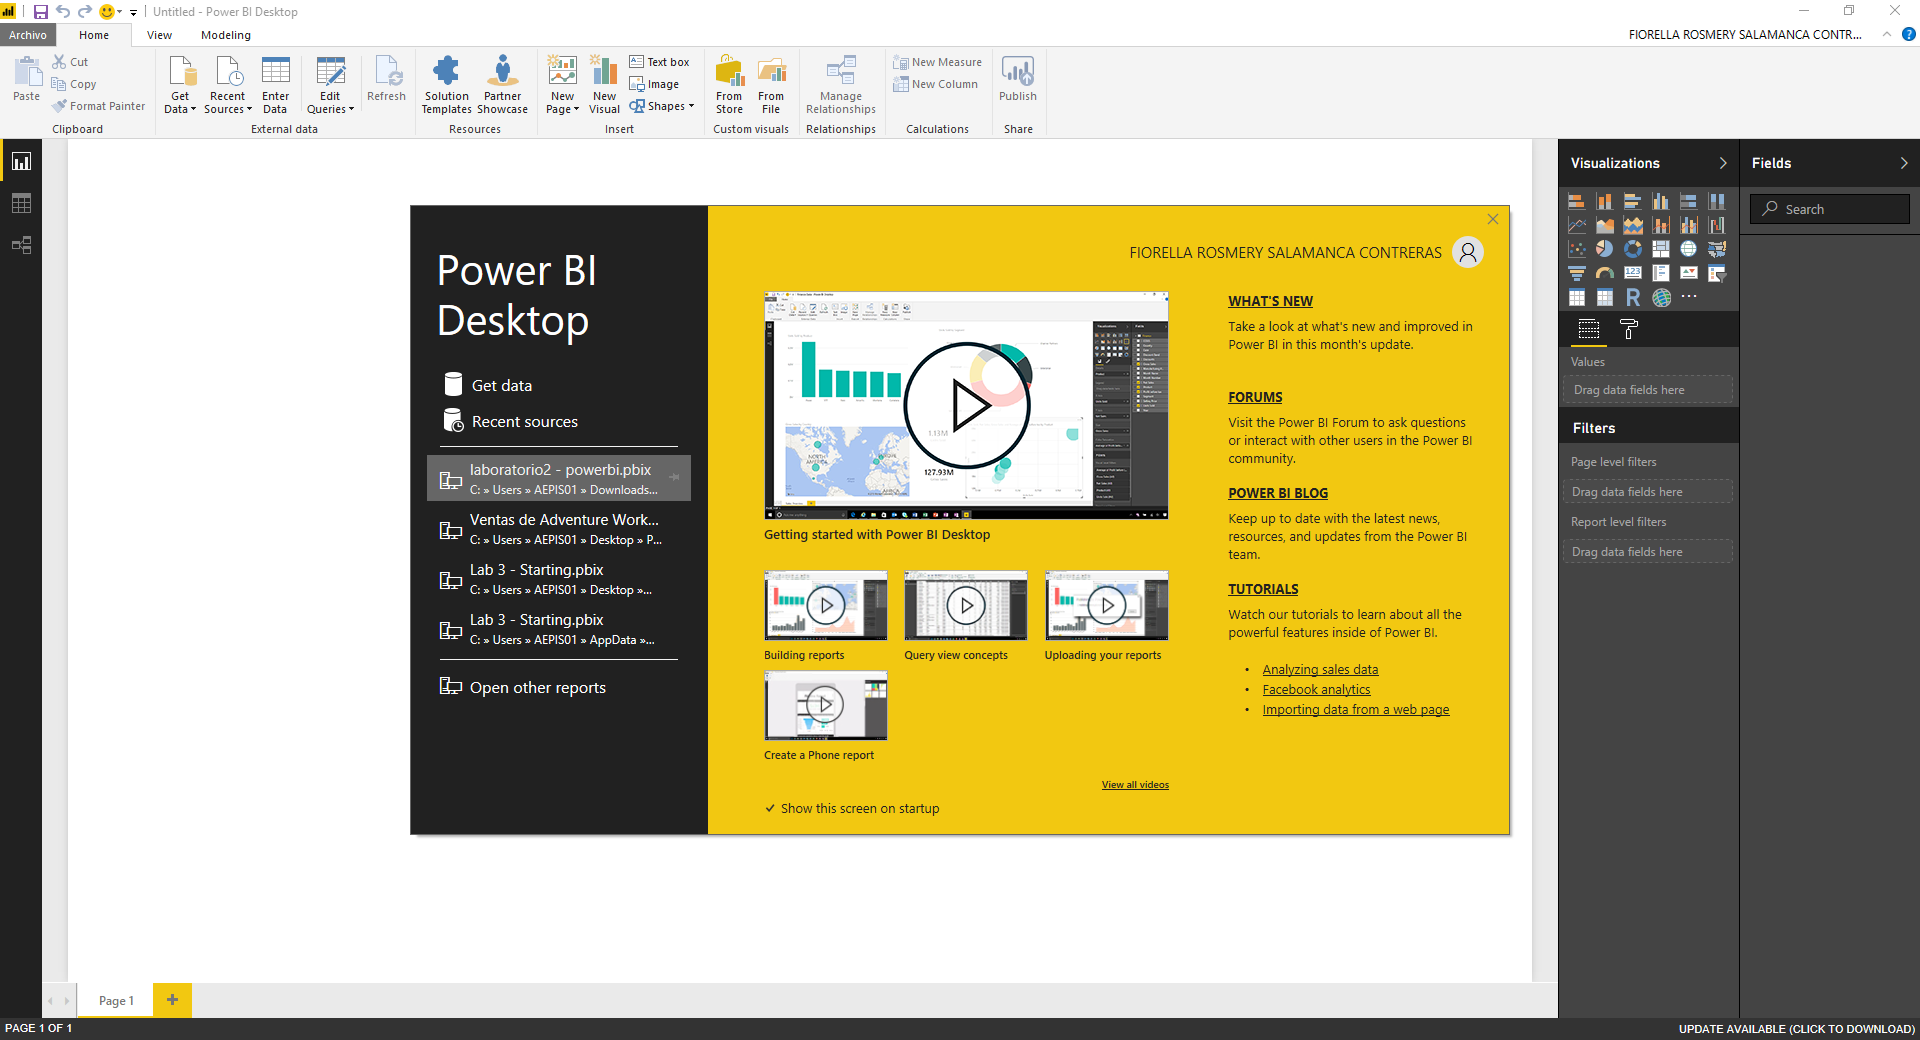
\includegraphics[width=15cm]{./Imagenes/Ejercicio1/Tarea2/3}
	\end{center}	
\section{Ejercicio 1: Conexión a datos de Power BI - Tarea 2: Conectarse a Datos Existentes en Azure} 

1. Open SQL Server Management Studio from the taskbar, and then connect to the MIA-SQL database engine instance by using Windows authentication.\\
2. On the File menu, point to Open, click Project/Solution, browse to the D:/Labfiles/Lab06/Starter/Project folder, and then double-click Project.ssmssln.

	\begin{center}
	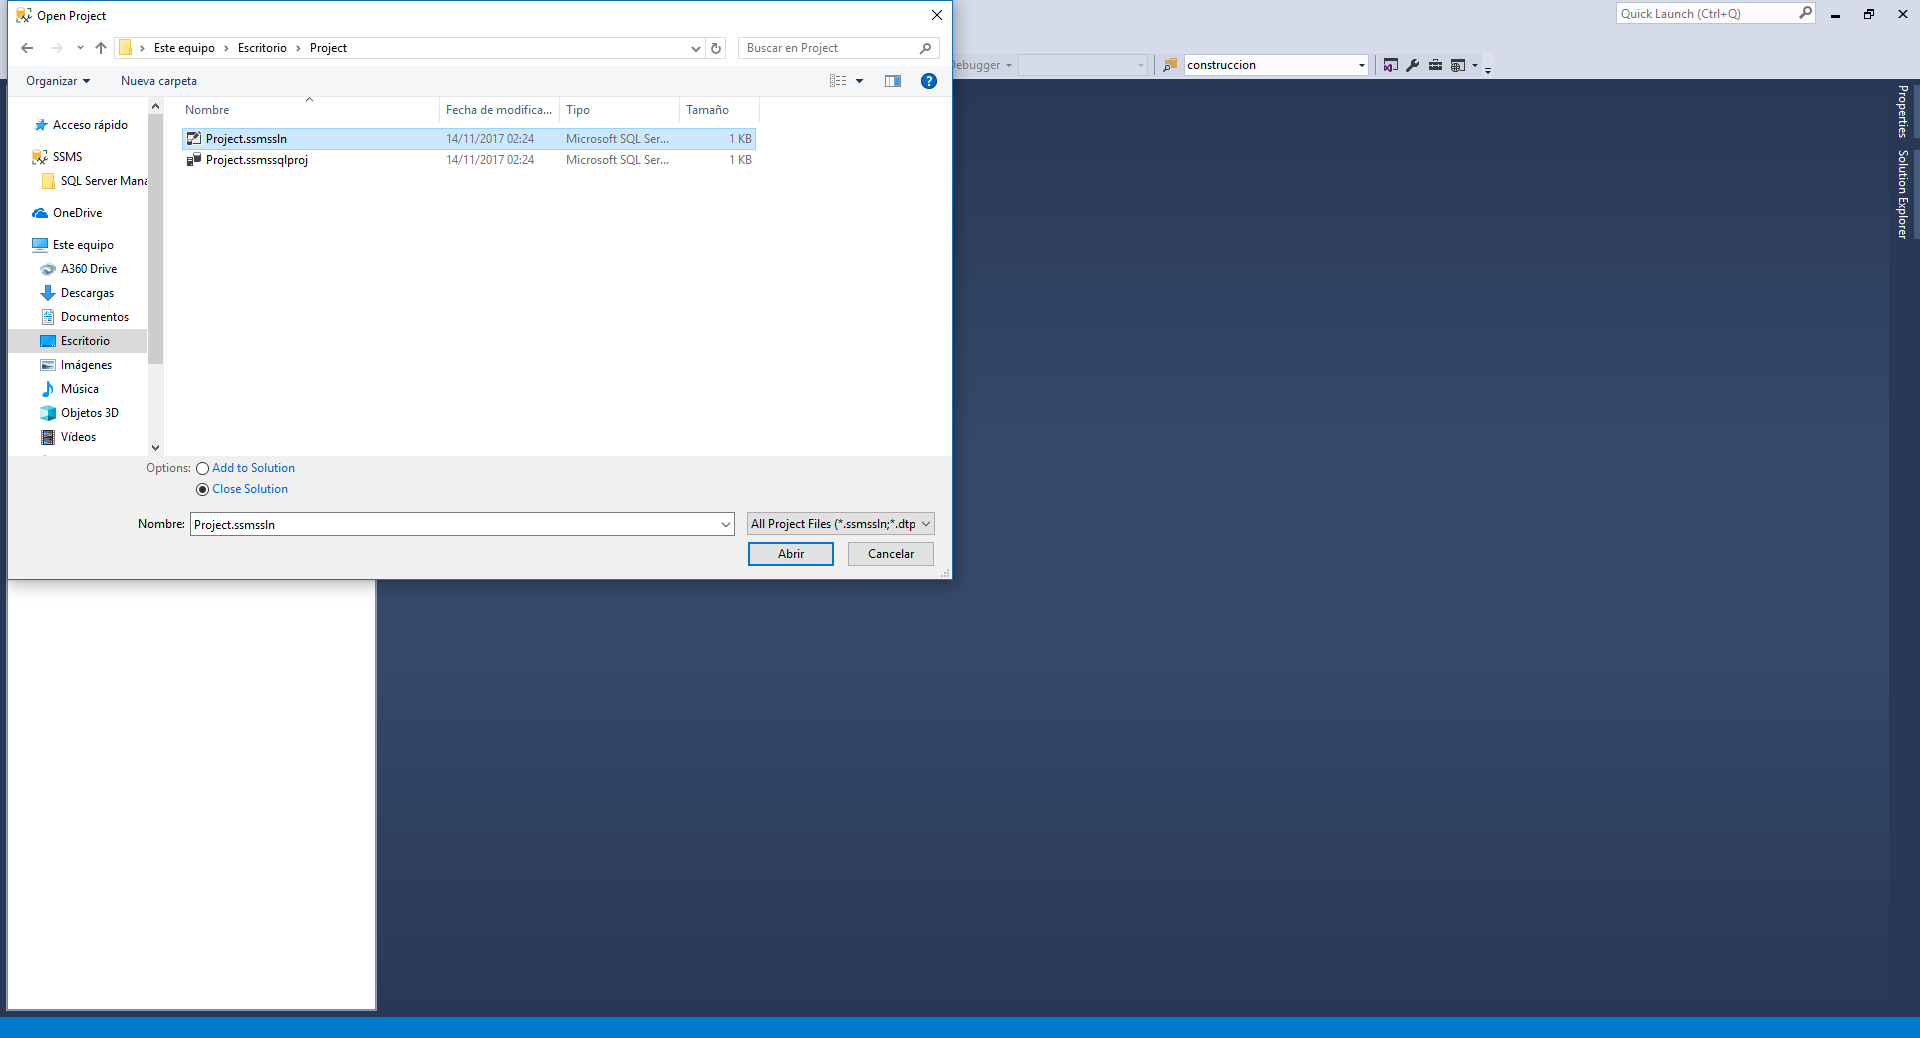
\includegraphics[width=17cm]{./Imagenes/Ejercicio1/Tarea2/1}
	\end{center}	

3. In Solution Explorer, expand Queries, and then double-click Lab Exercise 1.sql.\\

	\begin{center}
	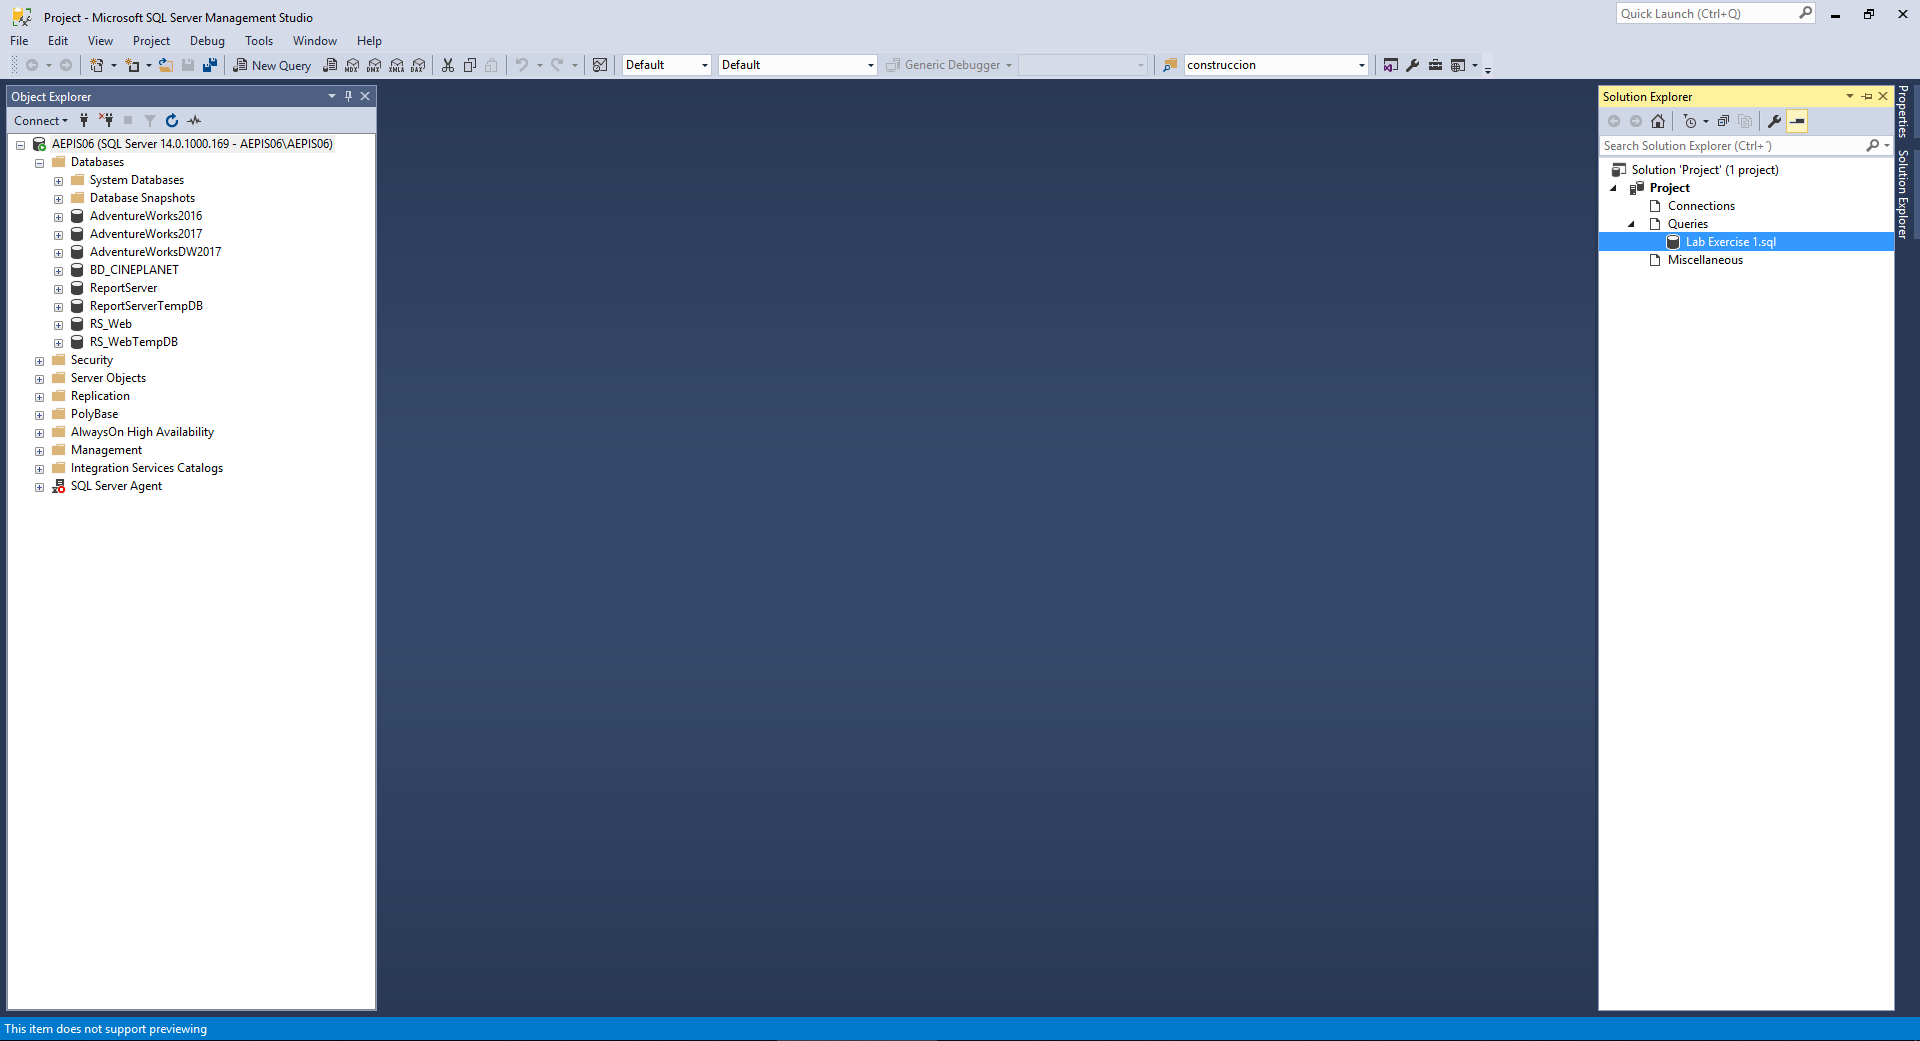
\includegraphics[width=17cm]{./Imagenes/Ejercicio1/Tarea2/2}
	\end{center}	

4. On the Desktop, double-click Power BI Desktop.\\
5. In the Power BI Desktop window, click Get Data.\\

	\begin{center}
	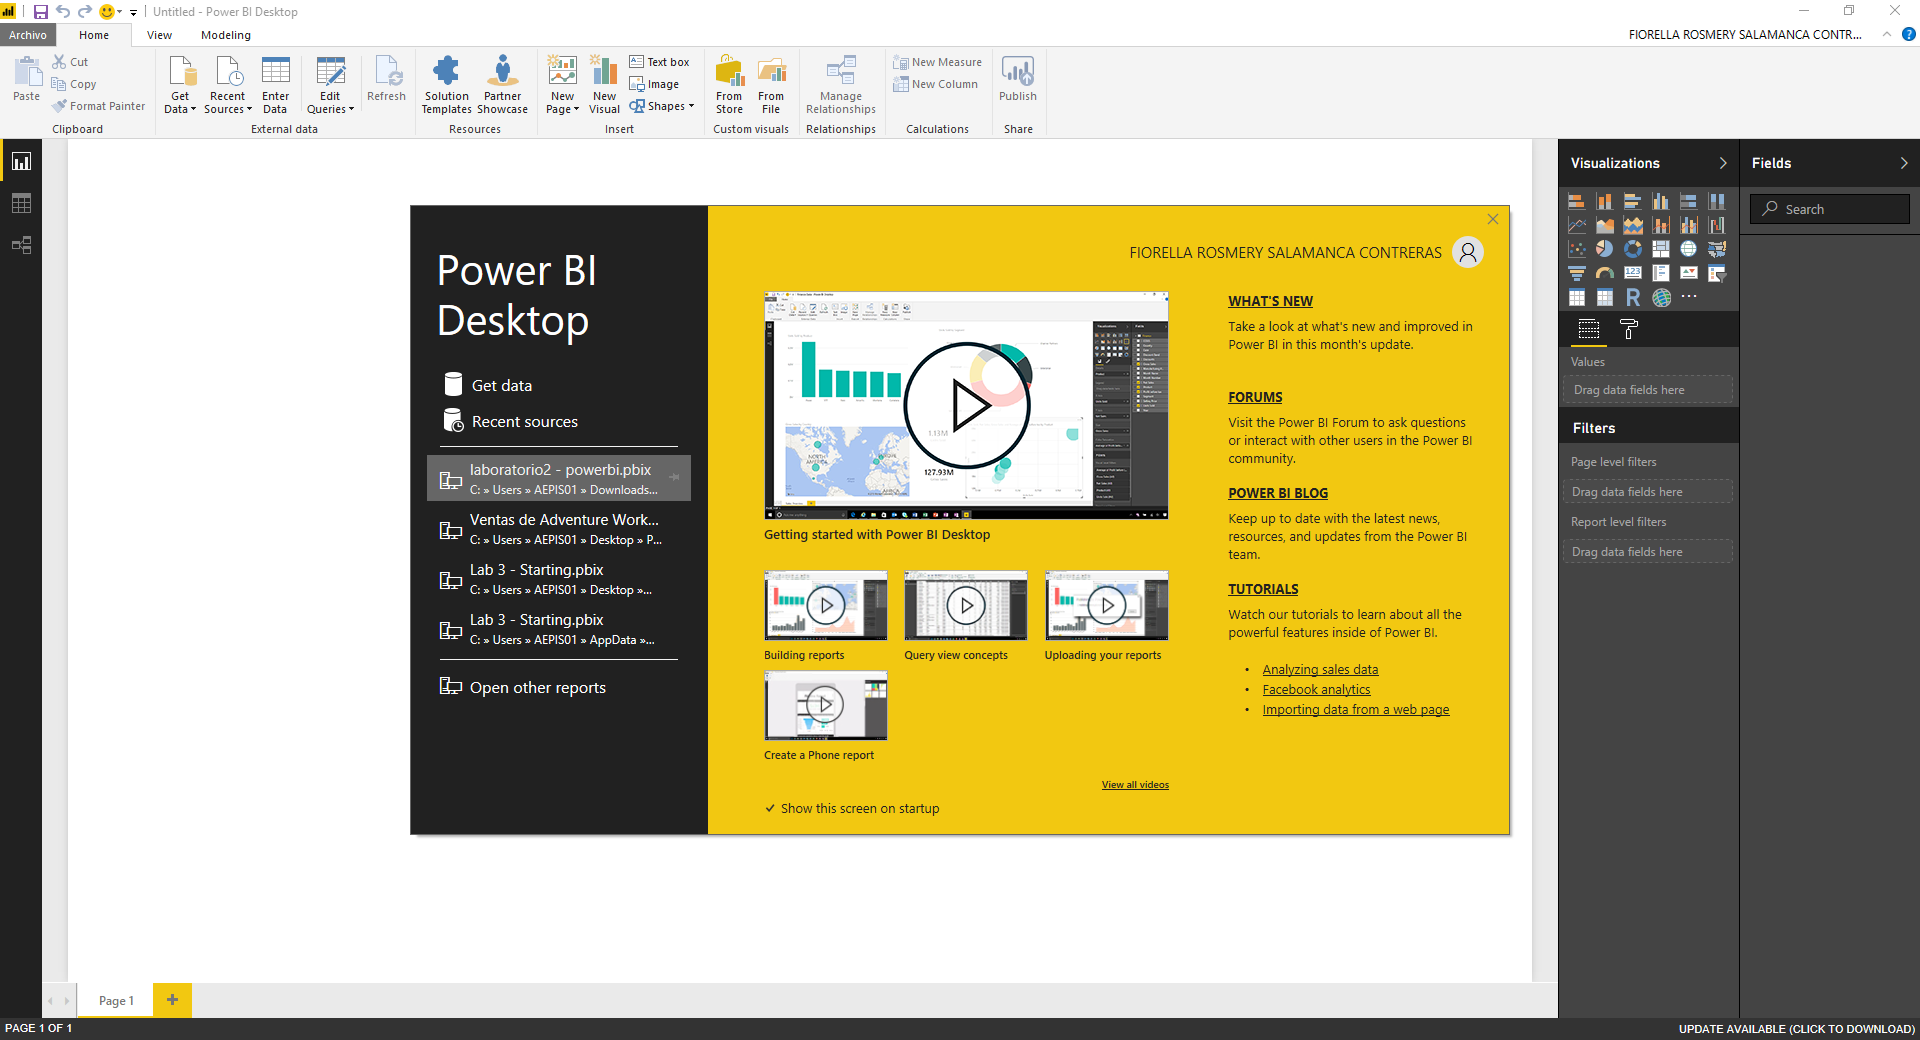
\includegraphics[width=17cm]{./Imagenes/Ejercicio1/Tarea2/3}
	\end{center}	

6. In the Get Data dialog box, click Microsoft Azure SQL database, and then click Connect\\

	\begin{center}
	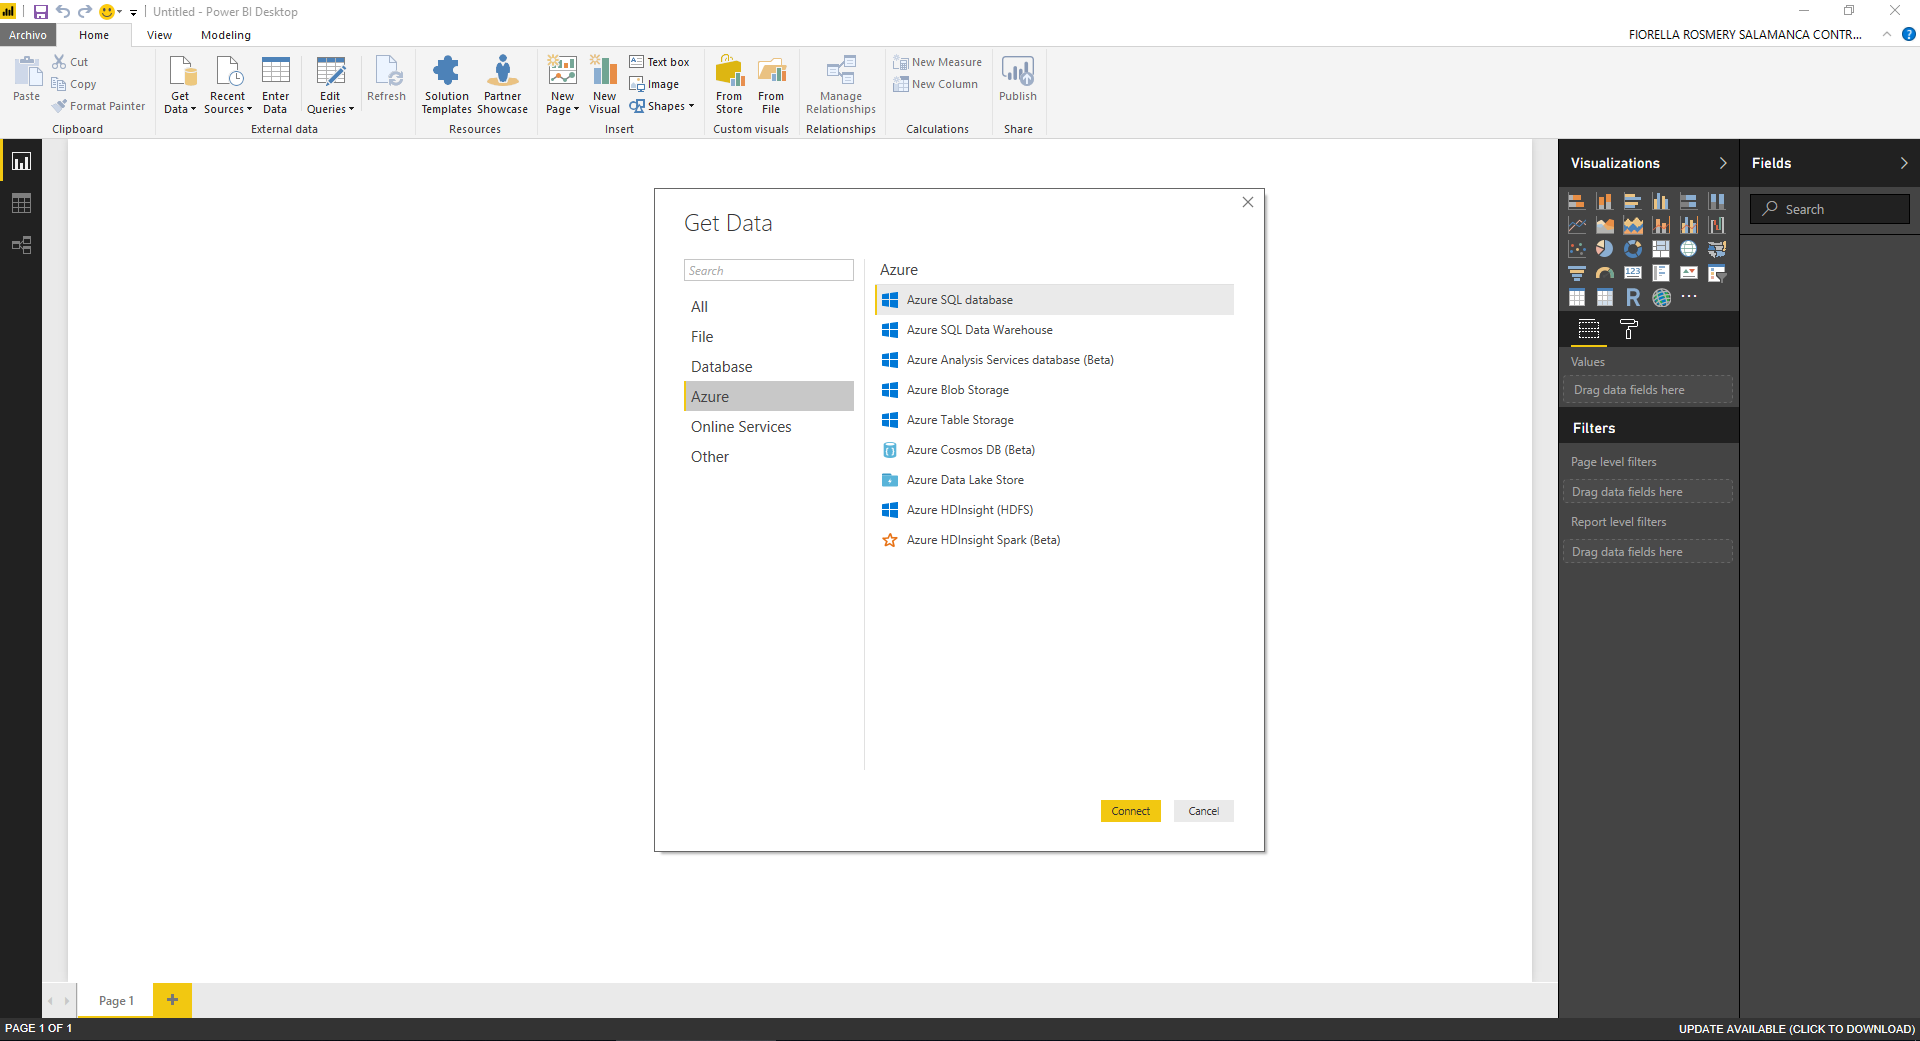
\includegraphics[width=17cm]{./Imagenes/Ejercicio1/Tarea2/4}
	\end{center}	

7. In the SQL Server database window, in the Server box, type the URL of the Azure server <Server Name>.database.windows.net.\\
8. In the Database (optional) box, type AdventureWorksLT.\\
9. Expand the Advanced options box.\\
10. In SQL Server Management Studio, copy the query under Task 1 in the Lab Exercise 1.sql query.\\
11. In Power BI Desktop, paste the query into the SQL statement (optional, requires database) box, and then click OK.\\

	\begin{center}
	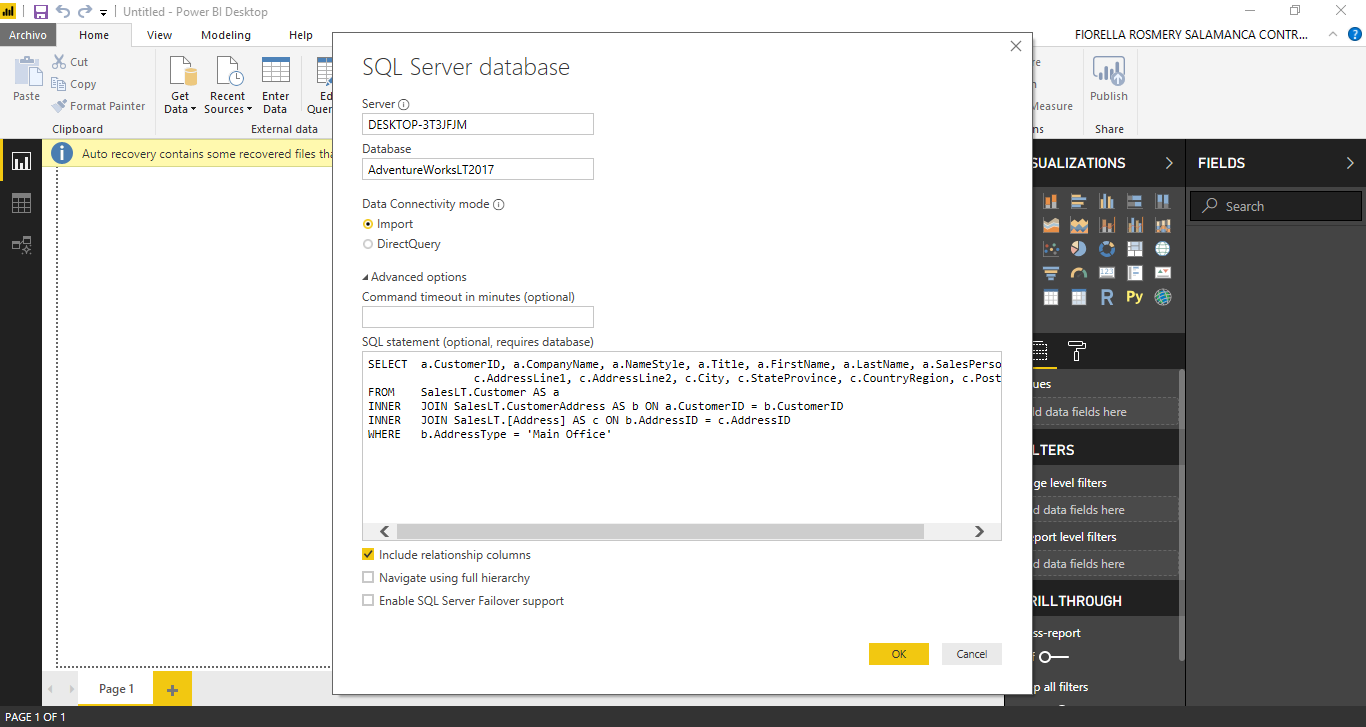
\includegraphics[width=17cm]{./Imagenes/Ejercicio1/Tarea2/5}
	\end{center}	

12. If the Access a SQL Server Database window appears, click Database, and then in the Username box, type Student, and in the Password box, type Pa\$\$w0rd. Click Connect.\\

	\begin{center}
	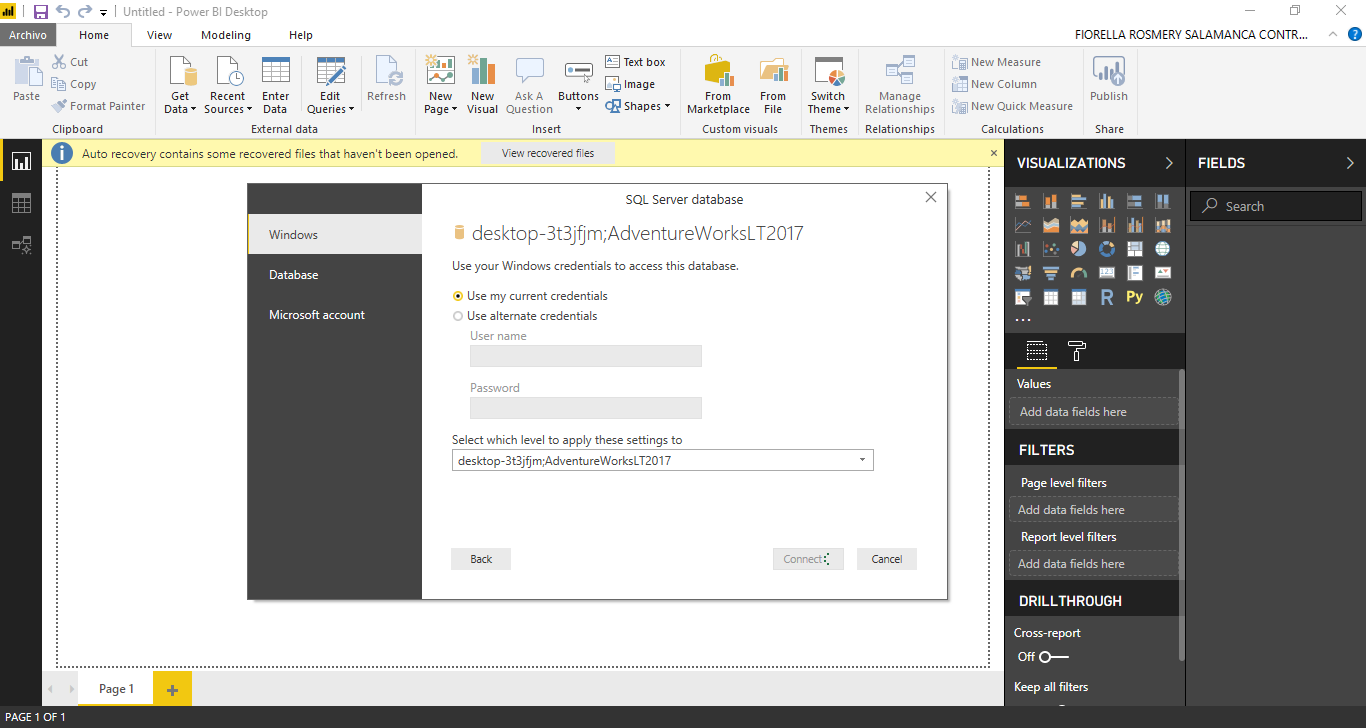
\includegraphics[width=17cm]{./Imagenes/Ejercicio1/Tarea2/6}
	\end{center}	

13. In the data preview window, click Load.\\

	\begin{center}
	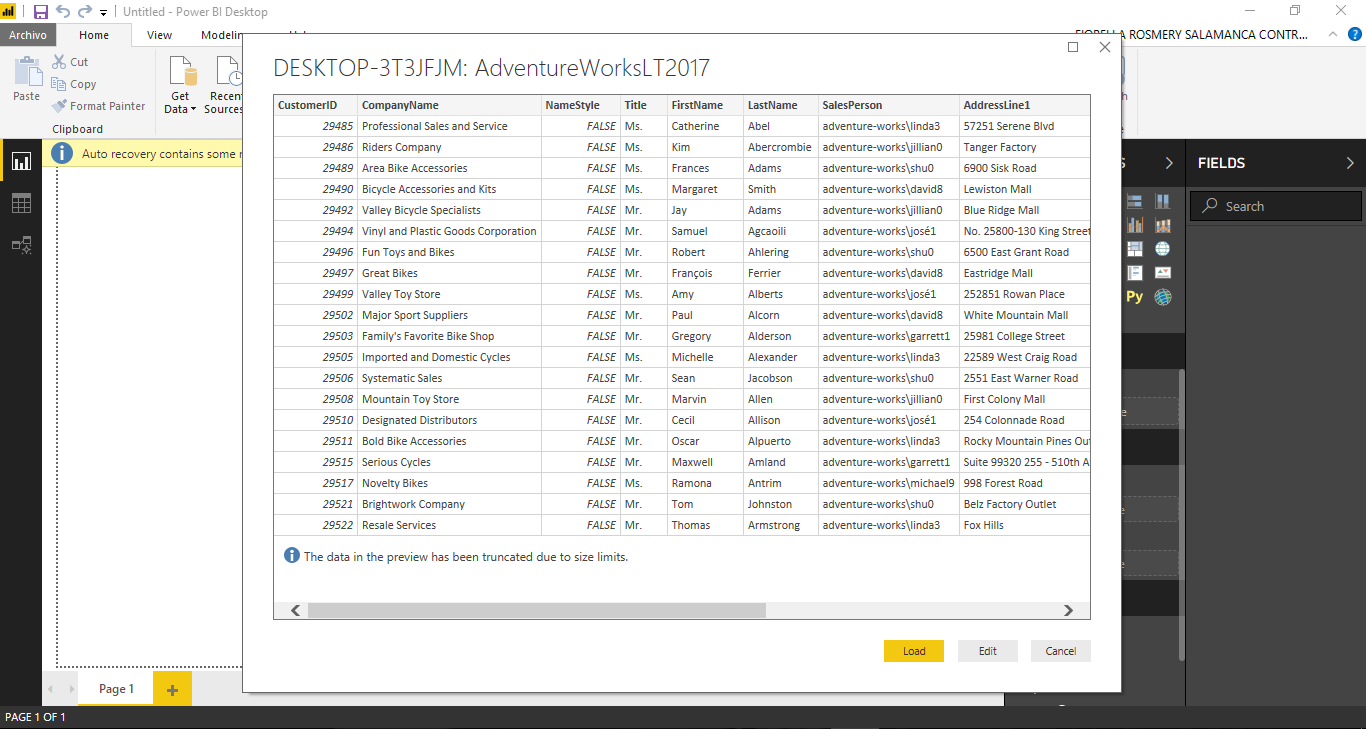
\includegraphics[width=17cm]{./Imagenes/Ejercicio1/Tarea2/7}
	\end{center}	

14. In Power BI Desktop, click Get Data then click More.\\
15. In the Get Data dialog box, click Microsoft Azure SQL database, and then click Connect.\\
16. In the SQL Server database window, in the Server box, type the URL of the Azure server <Server Name>.database.windows.net.\\
17. In the Database (optional) box, type AdventureWorksLT.\\
18. Expand the Advanced options box.\\
19. In SQL Server Management Studio, copy the query under Task 2 in the Lab Exercise 1.sql query.\\
20. In Power BI Desktop, paste the query into the SQL statement (optional, requires database) box, and then click OK.\\

	\begin{center}
	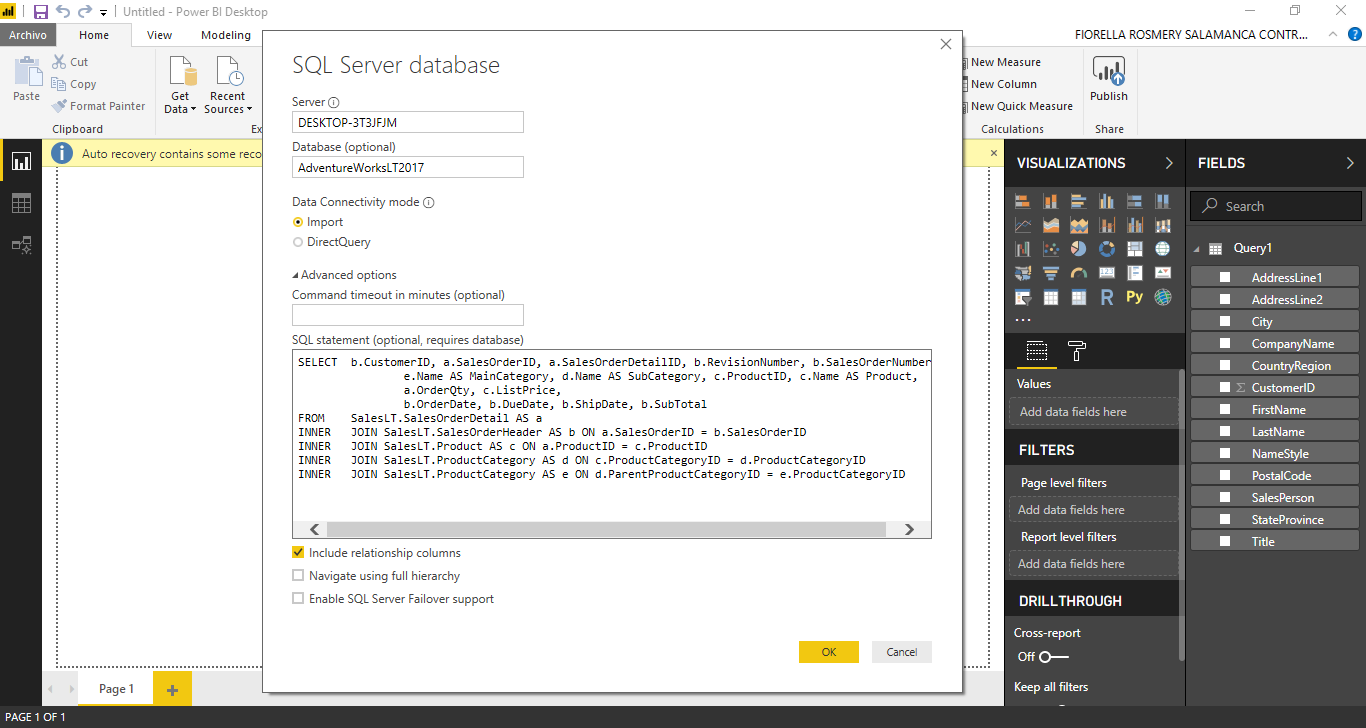
\includegraphics[width=17cm]{./Imagenes/Ejercicio1/Tarea2/8}
	\end{center}	

21. In the data preview window, click Load.\\

	\begin{center}
	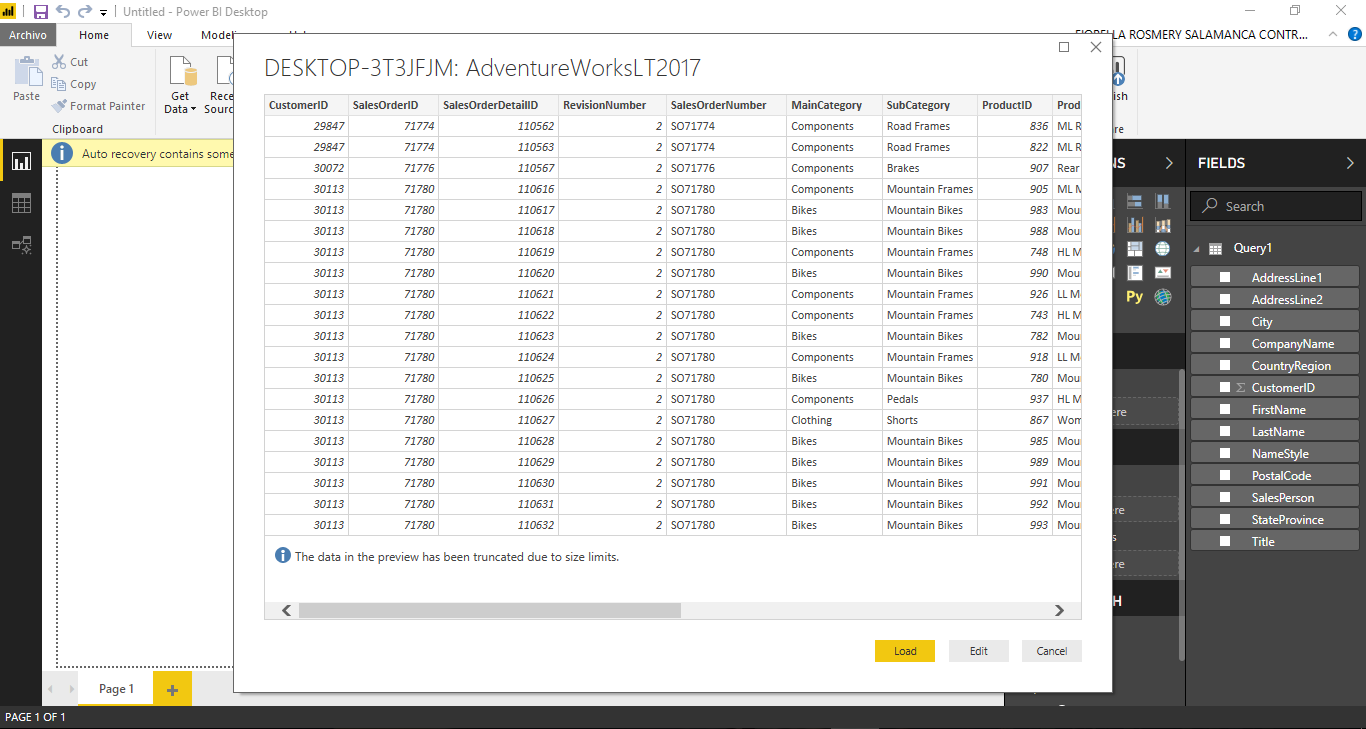
\includegraphics[width=17cm]{./Imagenes/Ejercicio1/Tarea2/9}
	\end{center}	

22. The window will close and return to the report, click Save.\\
23. In the Save As dialog box, navigate to D:/Labfiles/Lab06/Starter, in the File name box, type AdventureWorksLT Sales.pbix, and then click Save.\\

	\begin{center}
	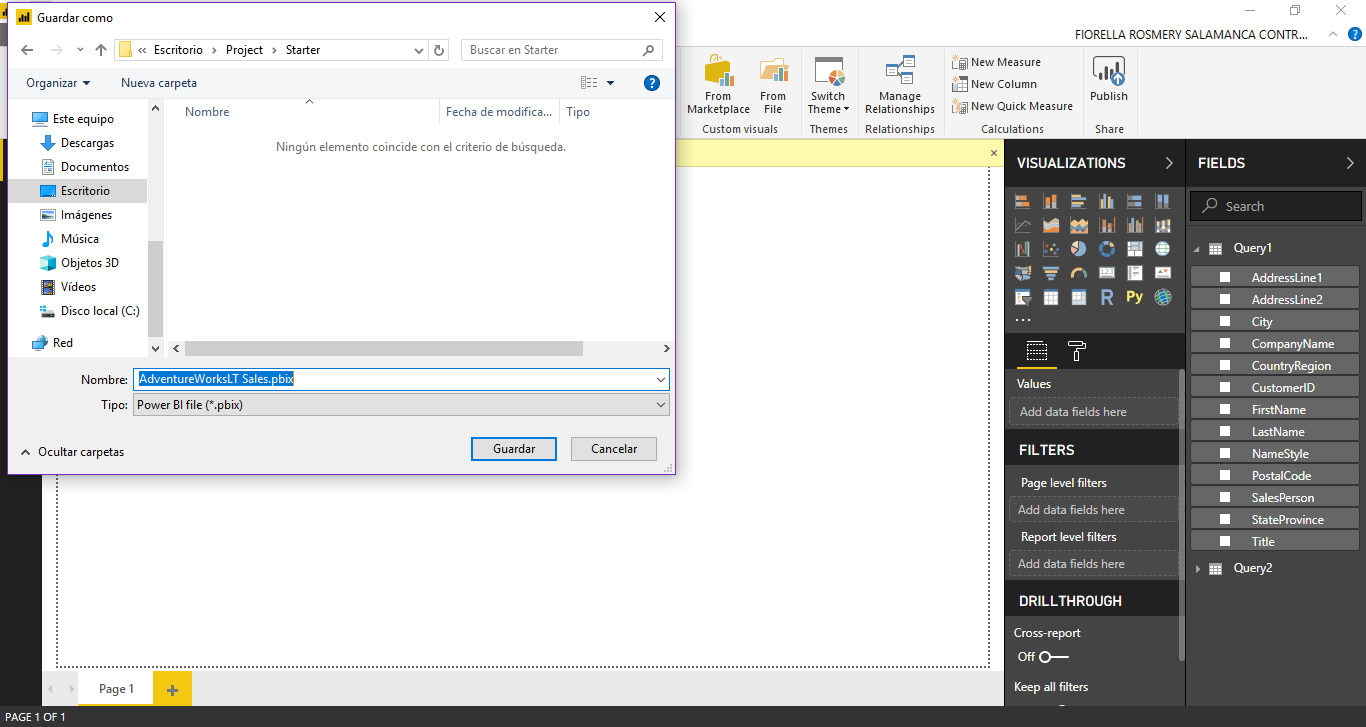
\includegraphics[width=17cm]{./Imagenes/Ejercicio1/Tarea2/10}
	\end{center}	

24. Leave Power BI Desktop open for the next task.\\
\section{Ejercicio 1: Conexión a datos de Power BI - Tarea 3: Forma de Datos} 

1. In the Fields pane, right-click Query1, click Rename, type Customers, and then press Enter.\\

	\begin{center}
	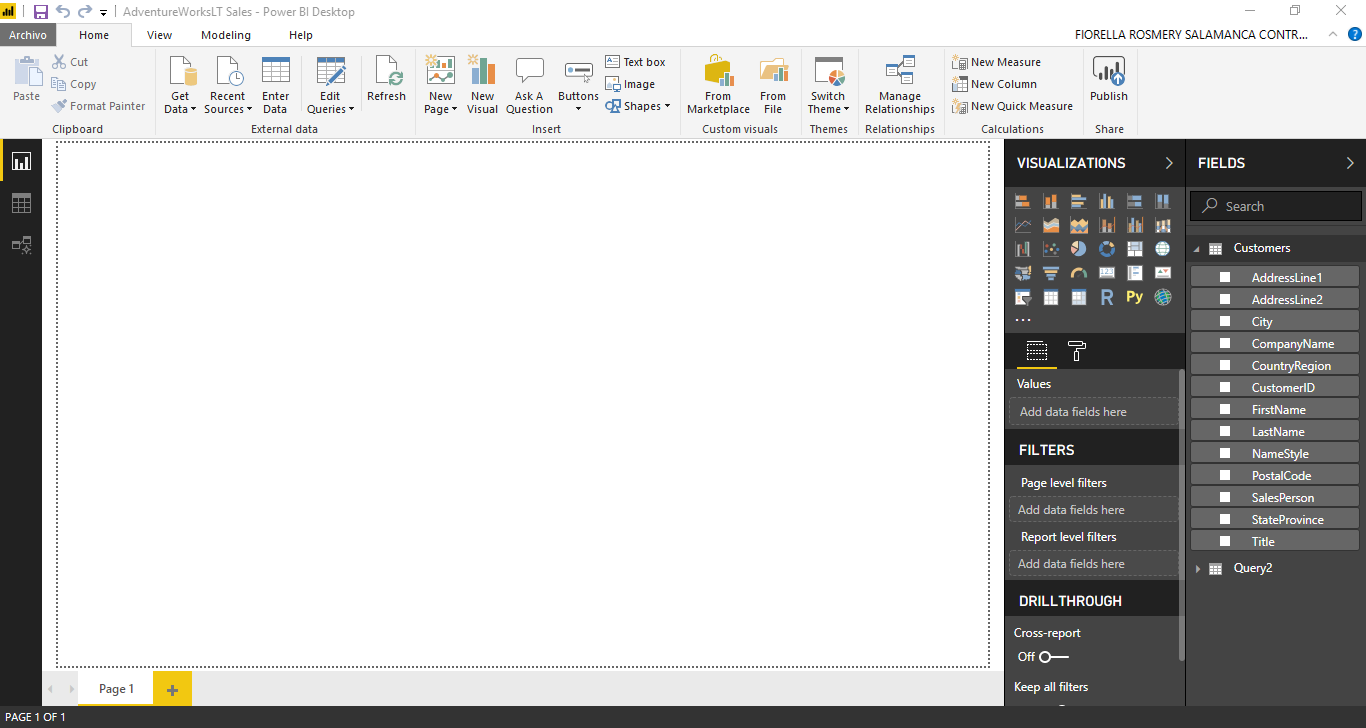
\includegraphics[width=17cm]{./Imagenes/Ejercicio1/Tarea3/1}
	\end{center}	

2. Right-click Query2, click Rename, type Sales, and then press Enter.\\

	\begin{center}
	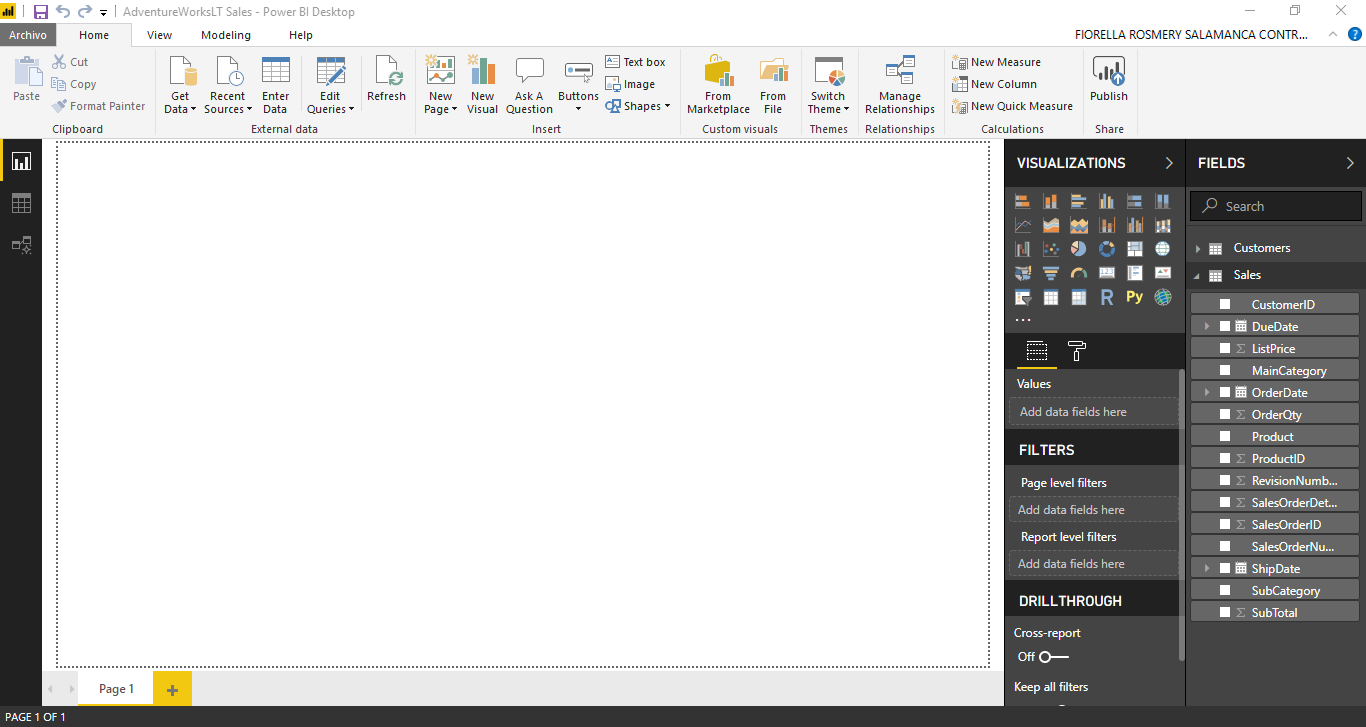
\includegraphics[width=17cm]{./Imagenes/Ejercicio1/Tarea3/2}
	\end{center}	

3. Expand the two tables to display all of the fields.\\
4. In the left navigation bar, click Data.\\
5. In the Fields pane, click the Customers table, if it is not already selected.\\
6. Right-click the NameStyle column, and click Delete.\\

	\begin{center}
	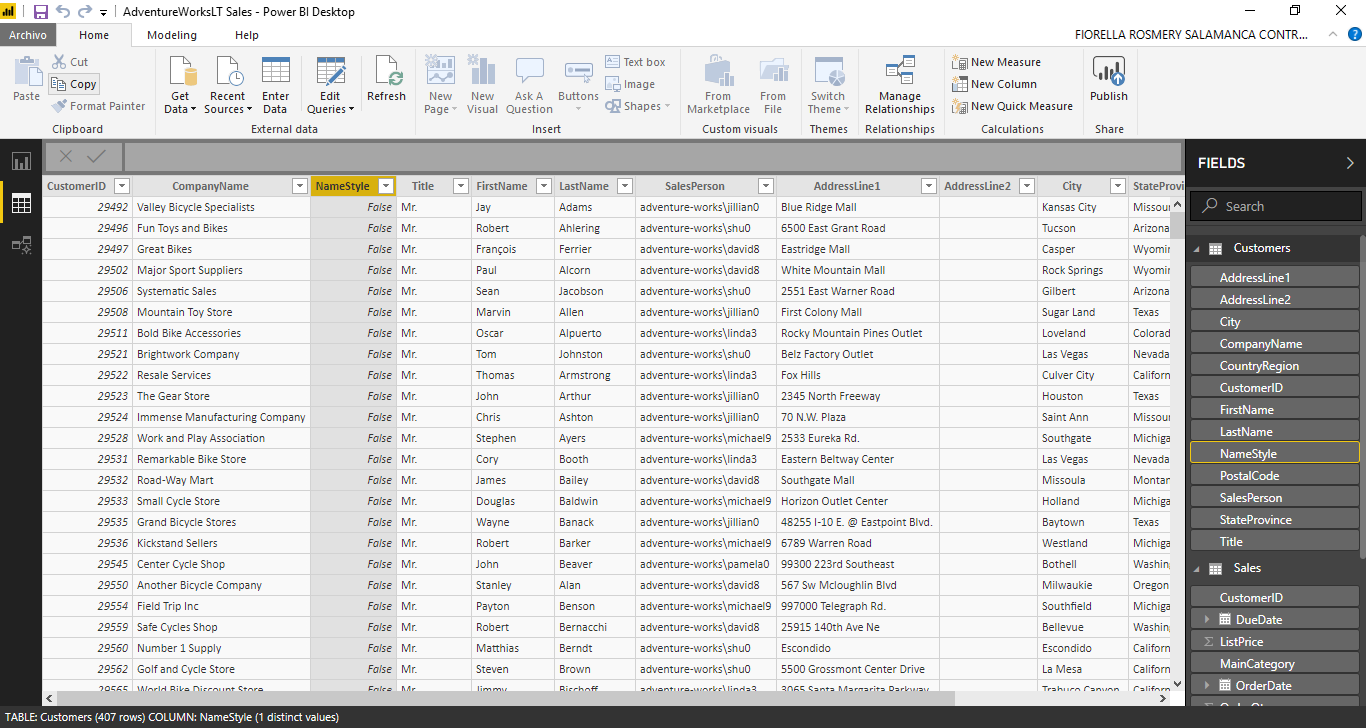
\includegraphics[width=17cm]{./Imagenes/Ejercicio1/Tarea3/3}
	\end{center}	

7. In the Delete Column dialog box, click Delete.\\

	\begin{center}
	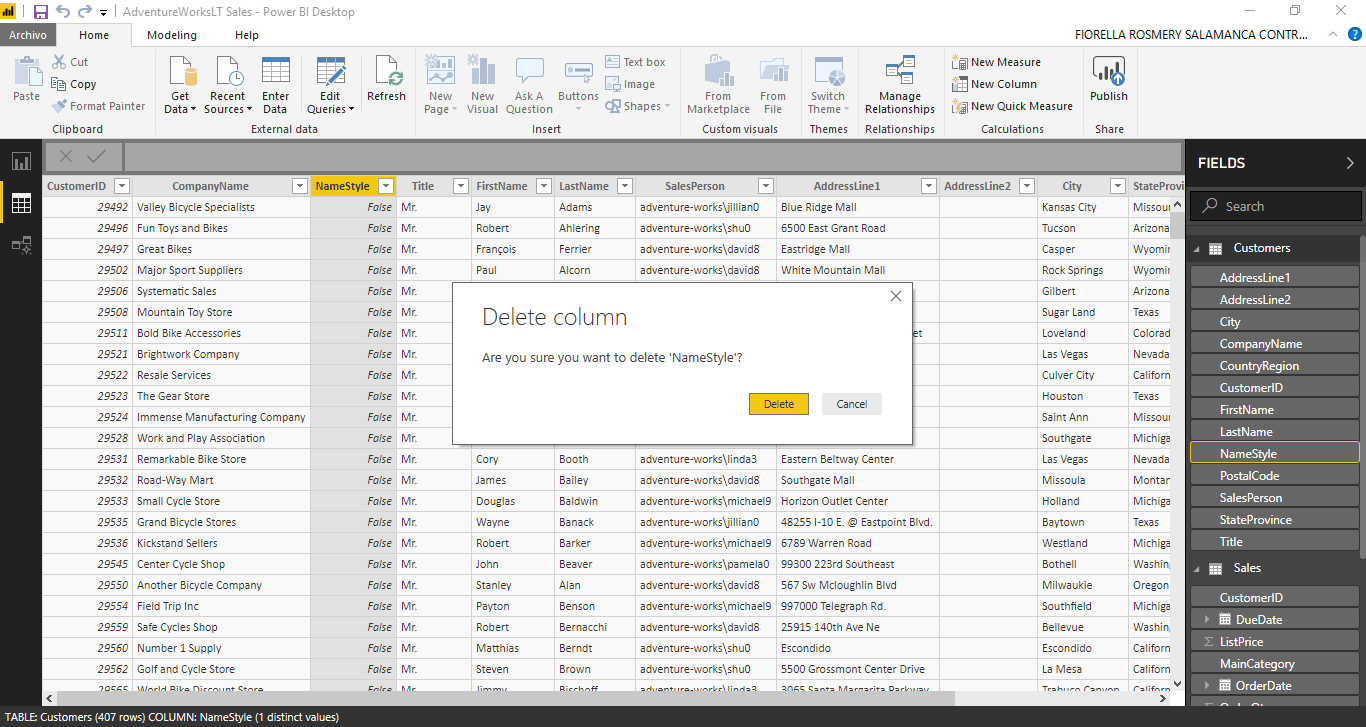
\includegraphics[width=17cm]{./Imagenes/Ejercicio1/Tarea3/4}
	\end{center}	

8. Right-click the SalesPerson column, and click Delete.\\

	\begin{center}
	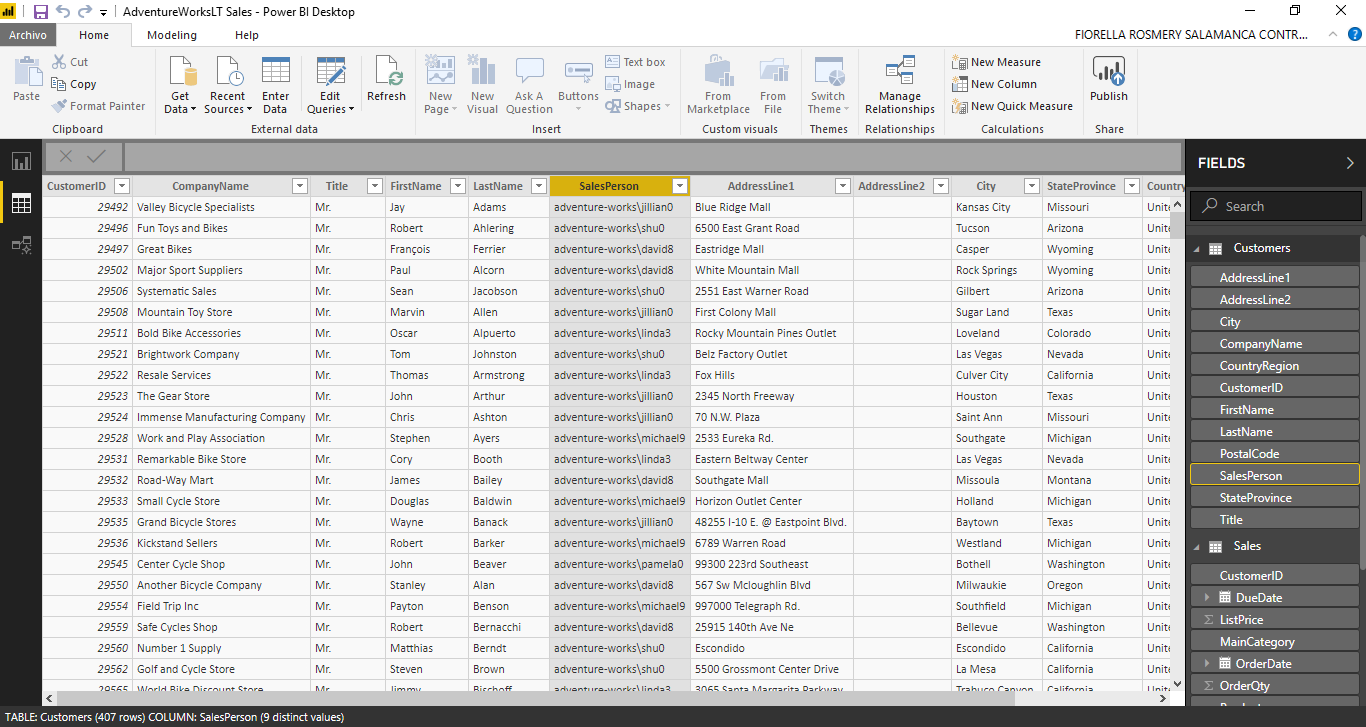
\includegraphics[width=17cm]{./Imagenes/Ejercicio1/Tarea3/5}
	\end{center}	

9. In the Delete Column dialog box, click Delete.\\

	\begin{center}
	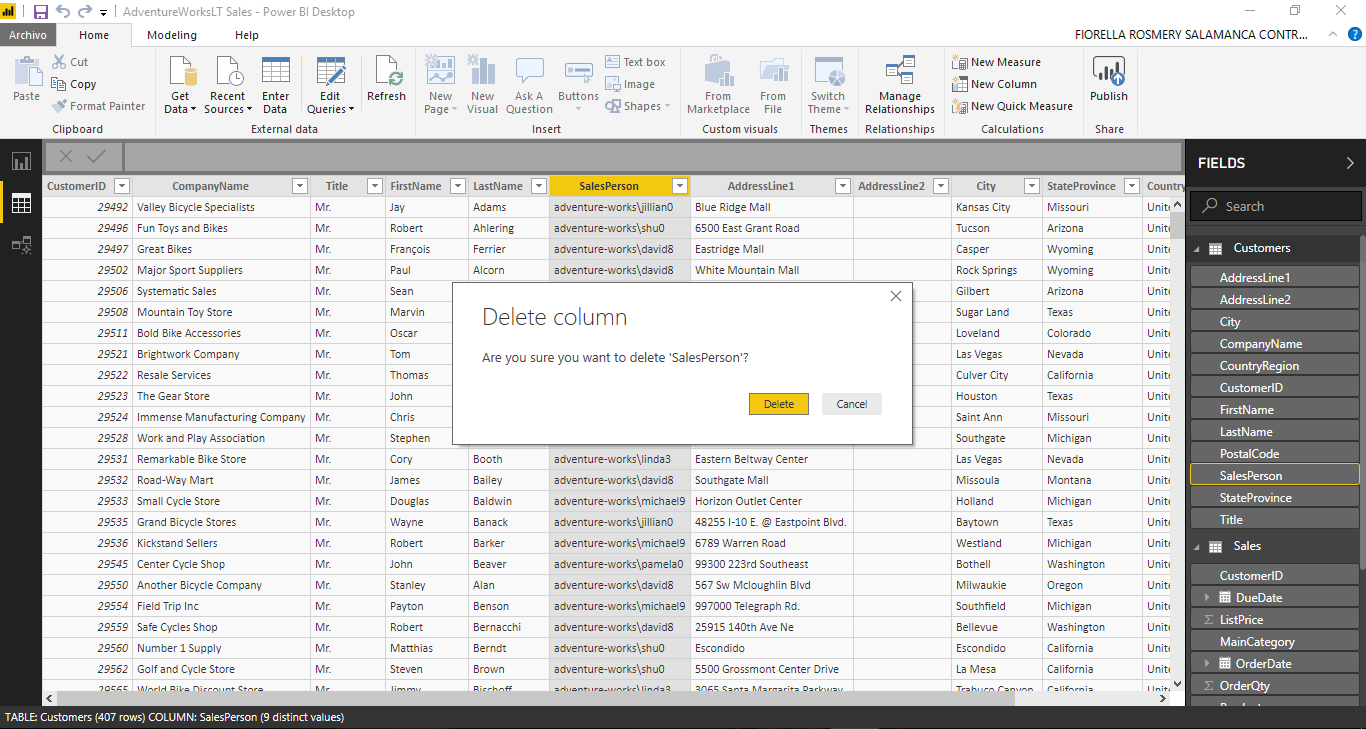
\includegraphics[width=17cm]{./Imagenes/Ejercicio1/Tarea3/6}
	\end{center}	

10. Right-click the CustomerID column, and then click Hide in Report View.\\

	\begin{center}
	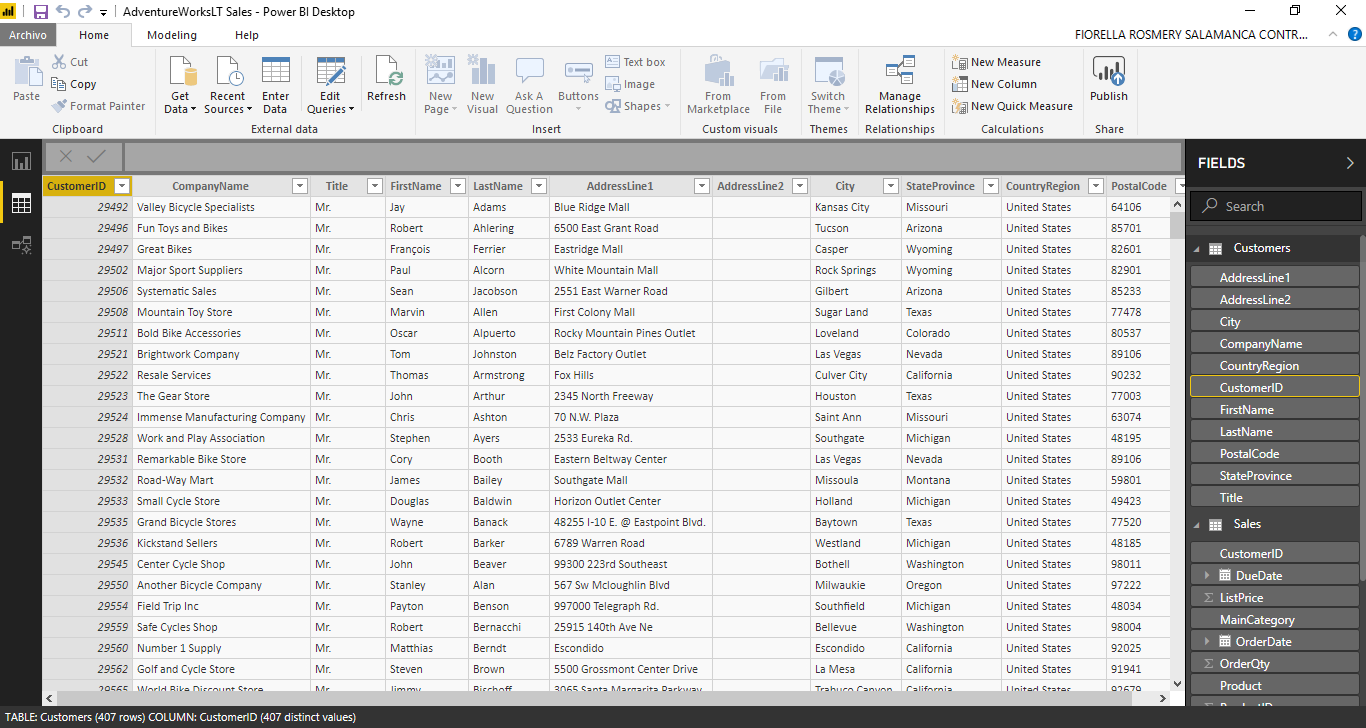
\includegraphics[width=17cm]{./Imagenes/Ejercicio1/Tarea3/7}
	\end{center}	

	\begin{center}
	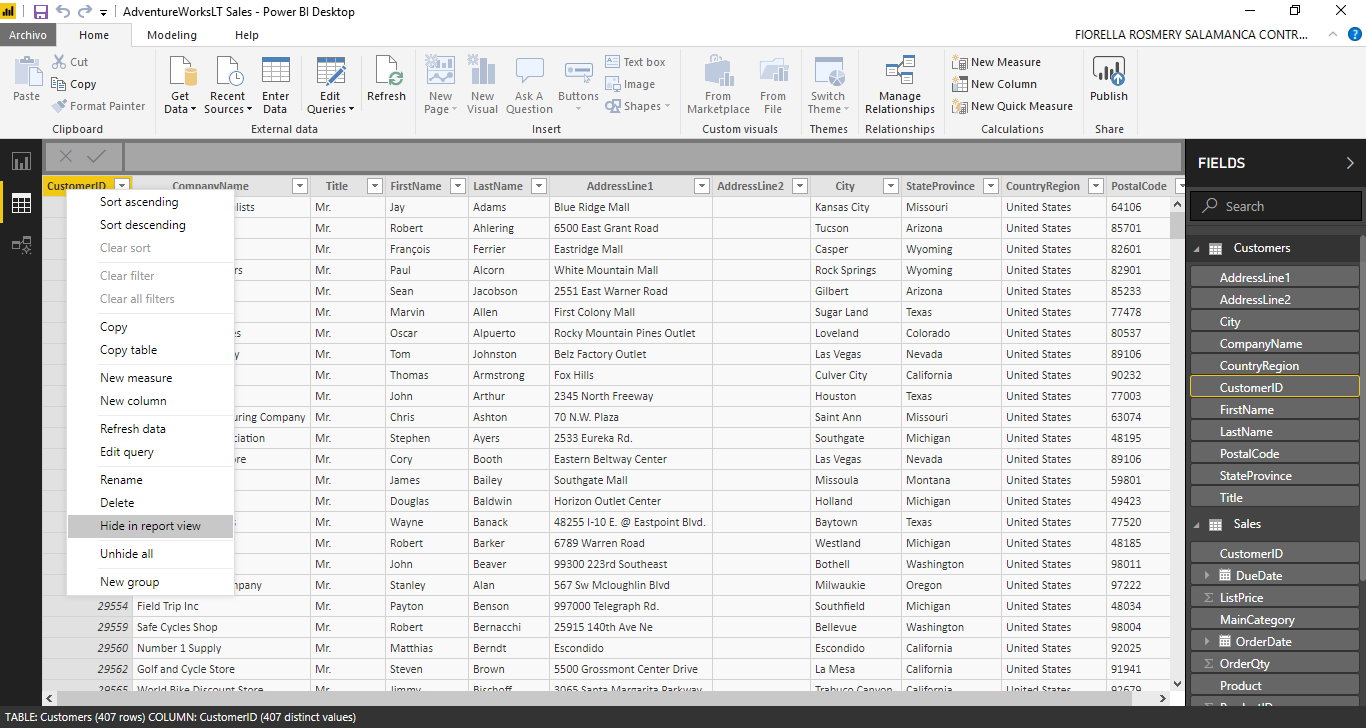
\includegraphics[width=17cm]{./Imagenes/Ejercicio1/Tarea3/8}
	\end{center}	

11. Click the AddressLine1 column header.\\

	\begin{center}
	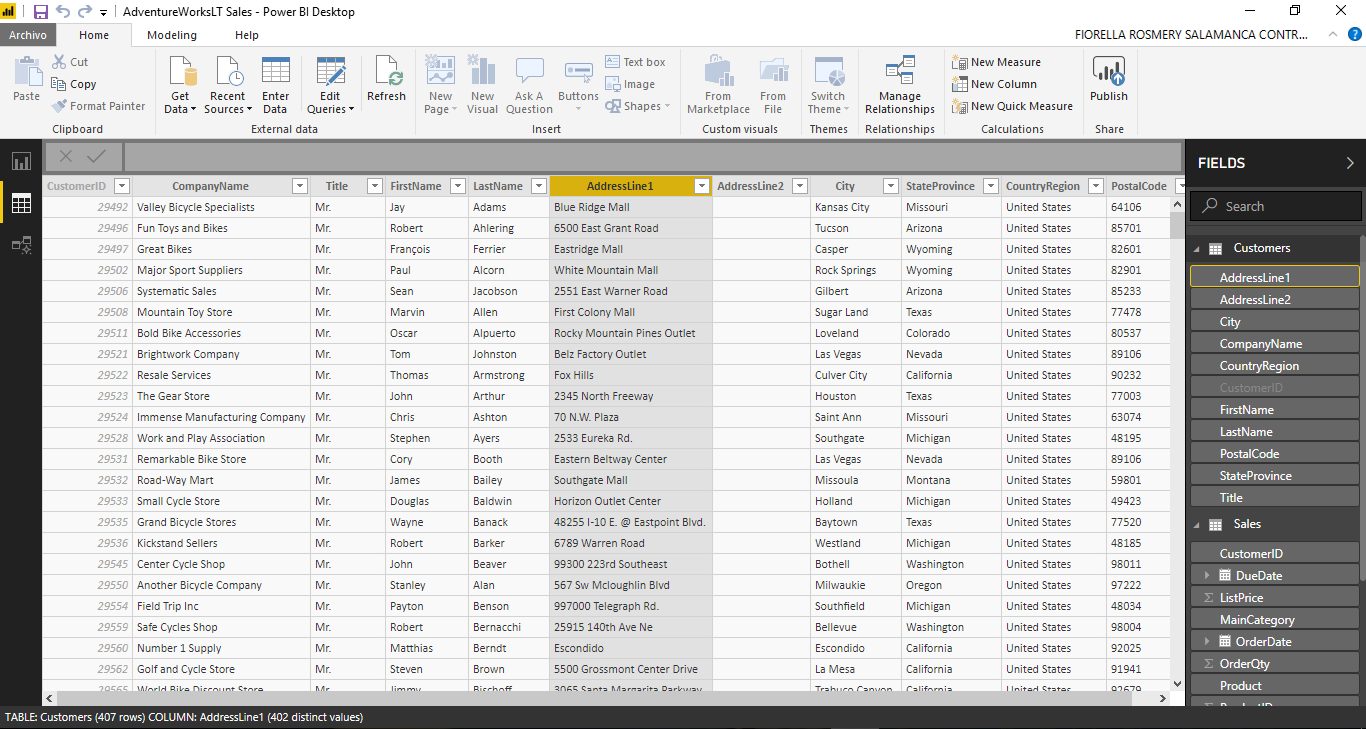
\includegraphics[width=17cm]{./Imagenes/Ejercicio1/Tarea3/9}
	\end{center}	

12. On the Modeling ribbon, in the Properties group, click Data Category: Uncategorized, and then click Address.\\

	\begin{center}
	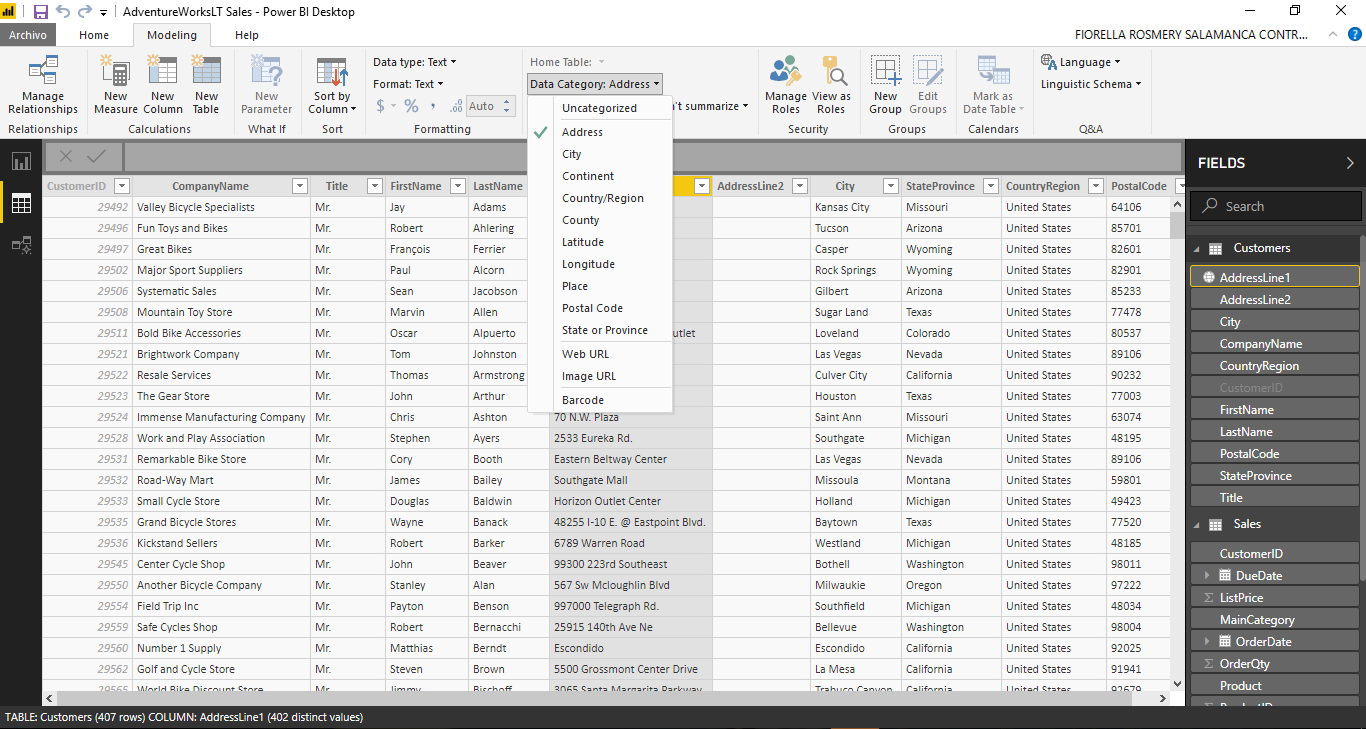
\includegraphics[width=17cm]{./Imagenes/Ejercicio1/Tarea3/10}
	\end{center}	

13. Click the City column header.\\

	\begin{center}
	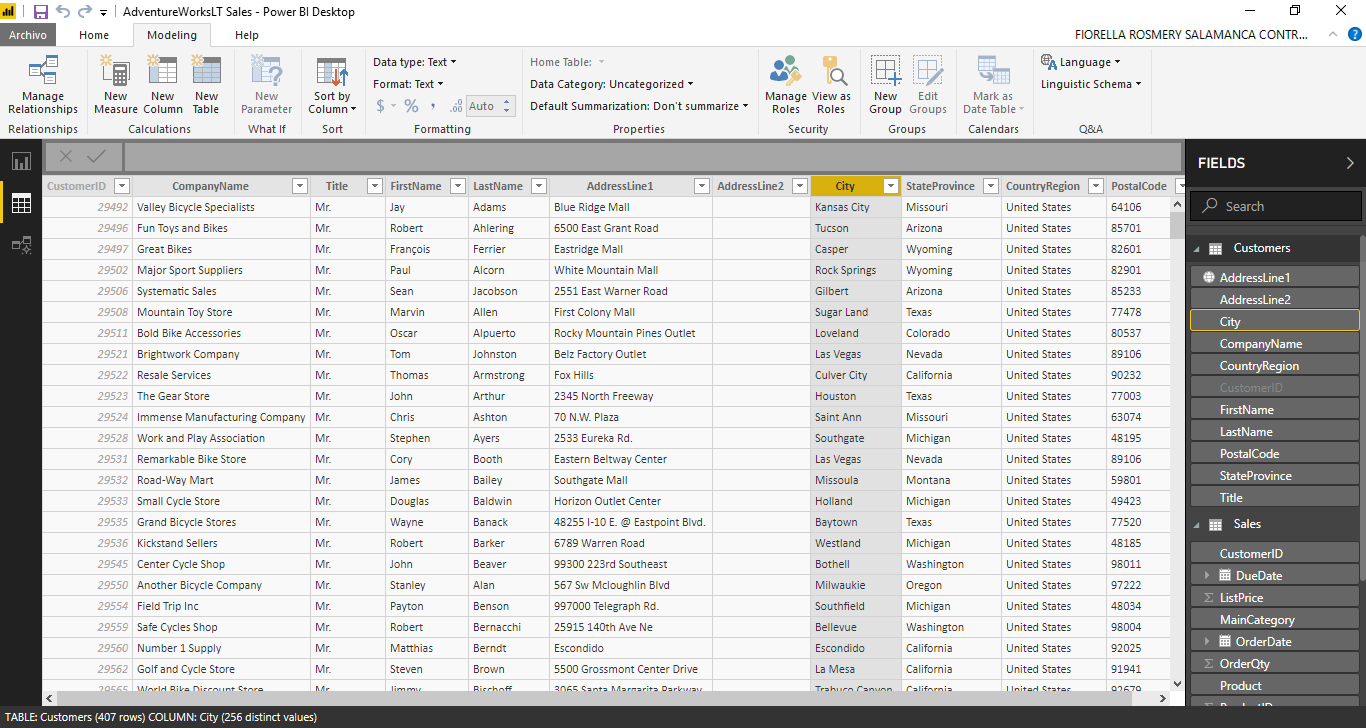
\includegraphics[width=17cm]{./Imagenes/Ejercicio1/Tarea3/11}
	\end{center}	

14. On the Modeling ribbon, in the Properties group, click Data Category: Uncategorized, and then click City.\\

	\begin{center}
	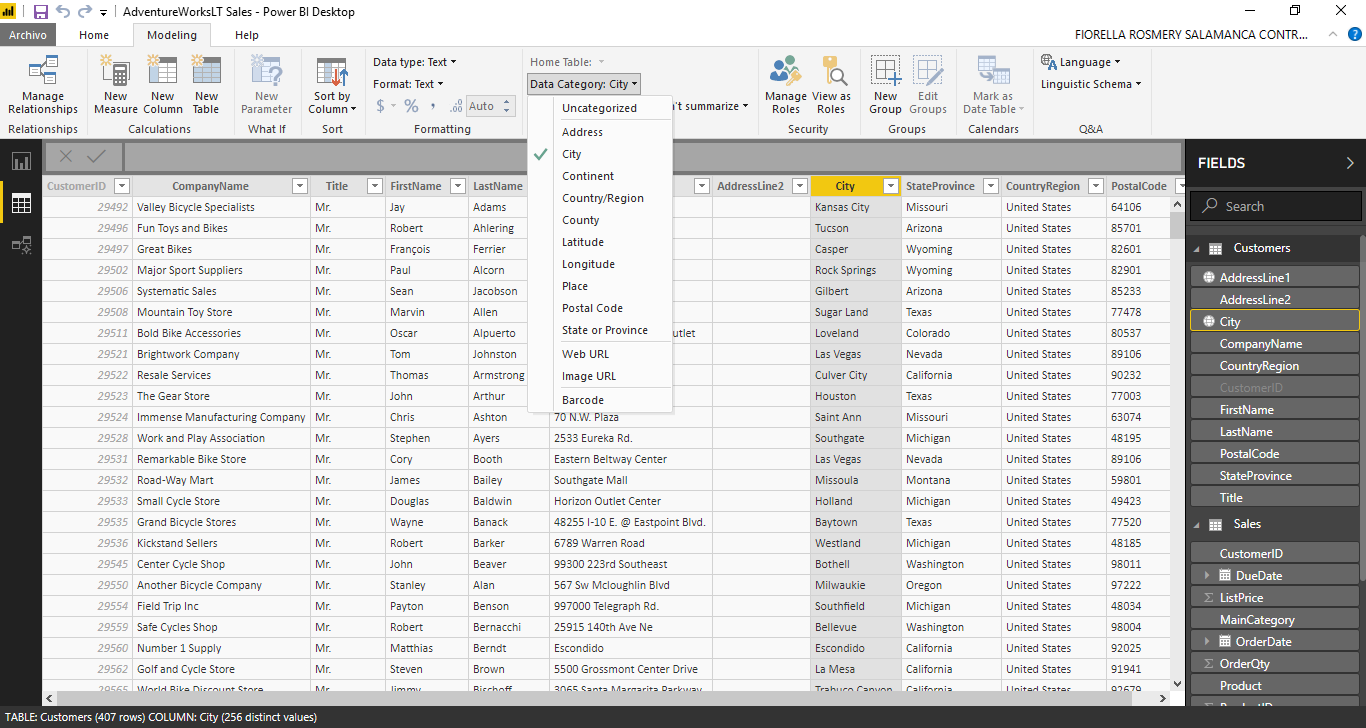
\includegraphics[width=17cm]{./Imagenes/Ejercicio1/Tarea3/12}
	\end{center}	

15. Click the StateProvince column header.\\

	\begin{center}
	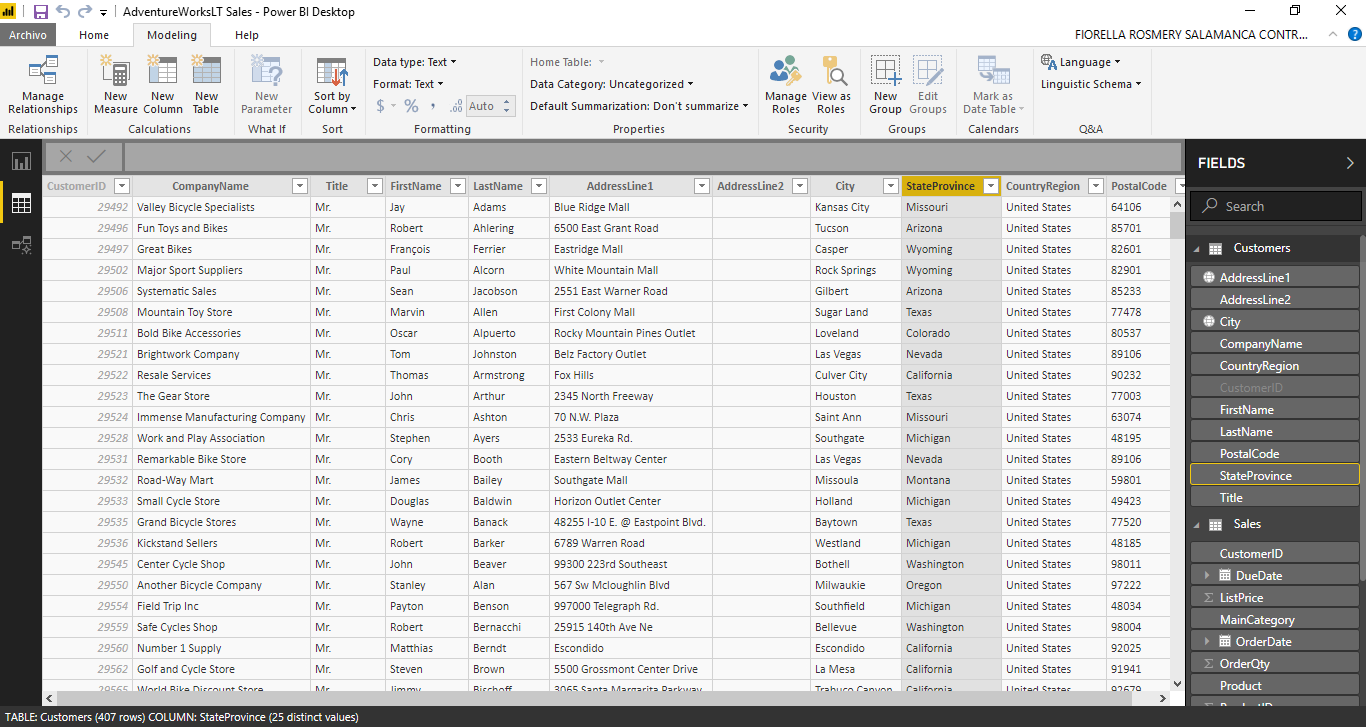
\includegraphics[width=17cm]{./Imagenes/Ejercicio1/Tarea3/13}
	\end{center}	

16. On the Modeling ribbon, in the Properties group, click Data Category: Uncategorized, and then click State or Province.\\

	\begin{center}
	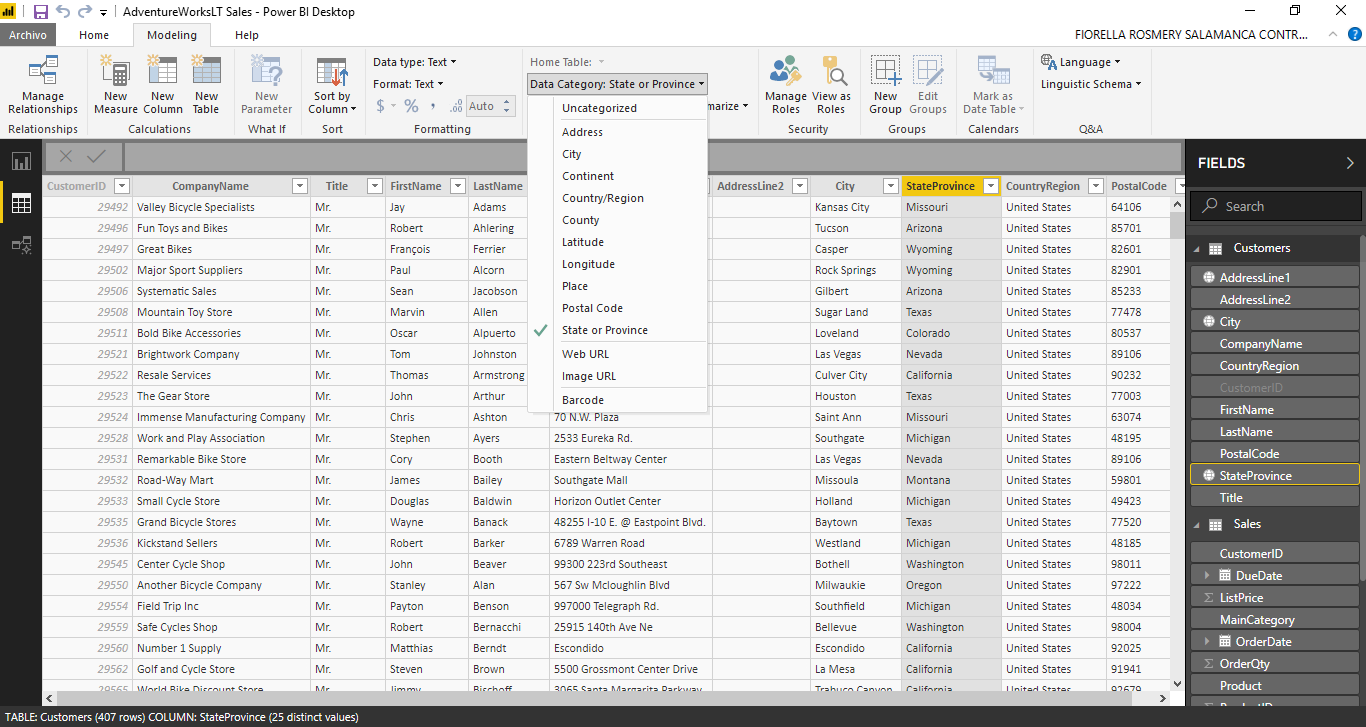
\includegraphics[width=17cm]{./Imagenes/Ejercicio1/Tarea3/14}
	\end{center}	

17. Click the CountryRegion column header.\\

	\begin{center}
	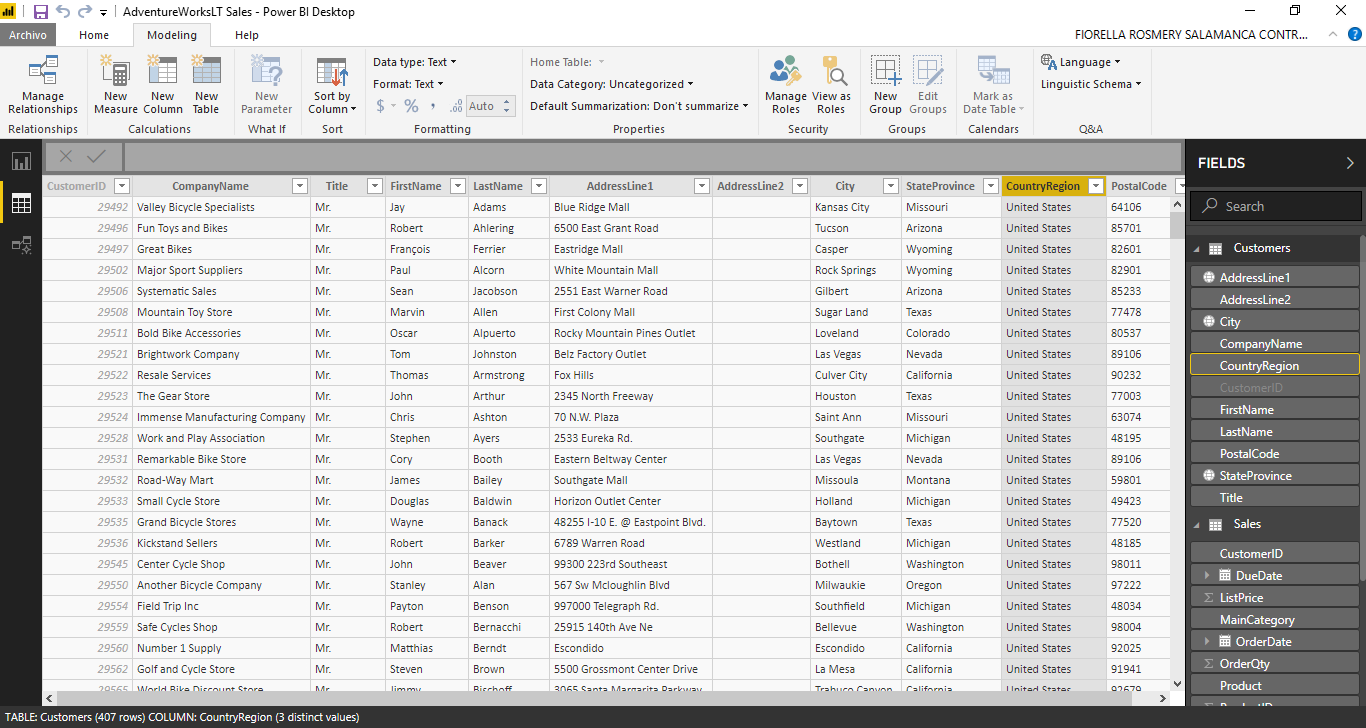
\includegraphics[width=17cm]{./Imagenes/Ejercicio1/Tarea3/15}
	\end{center}	

18. On the Modeling ribbon, in the Properties group, click Data Category: Uncategorized, and then click Country/Region.\\

	\begin{center}
	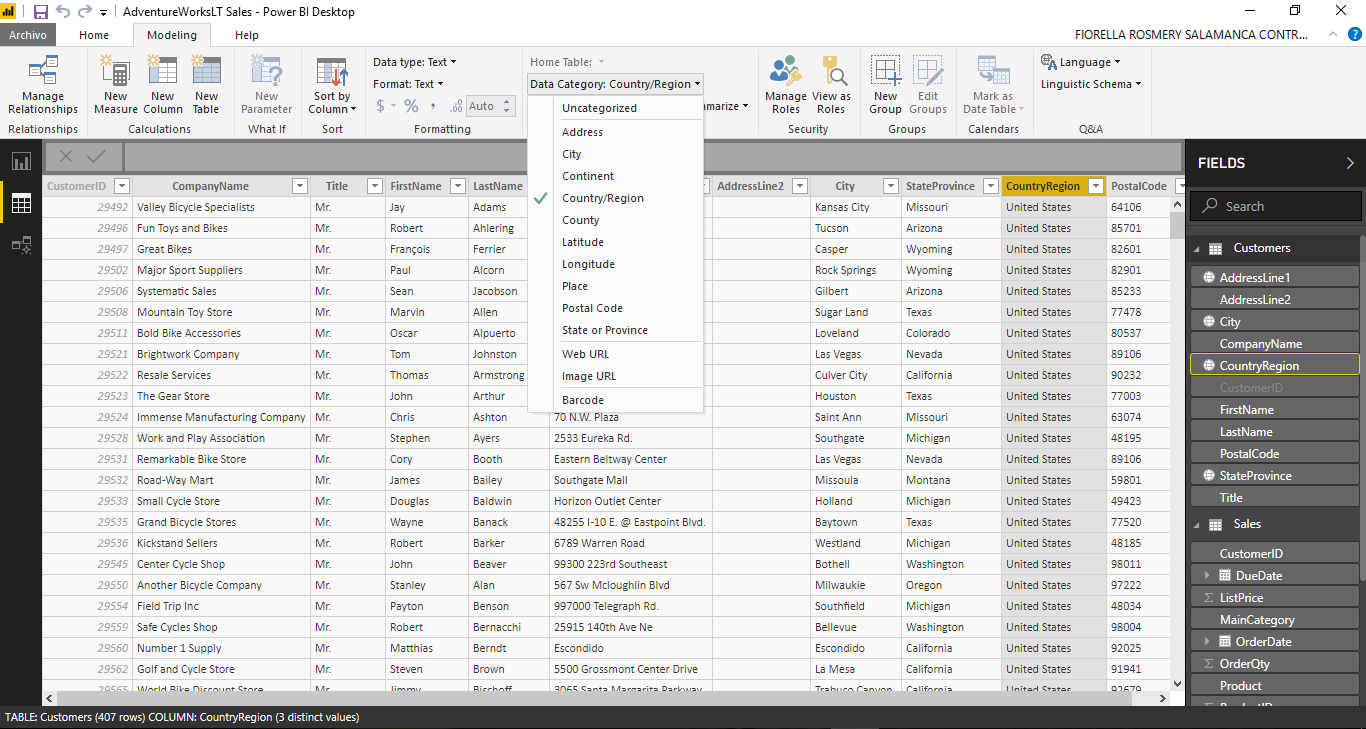
\includegraphics[width=17cm]{./Imagenes/Ejercicio1/Tarea3/16}
	\end{center}	

19. Click the PostalCode column header.\\

	\begin{center}
	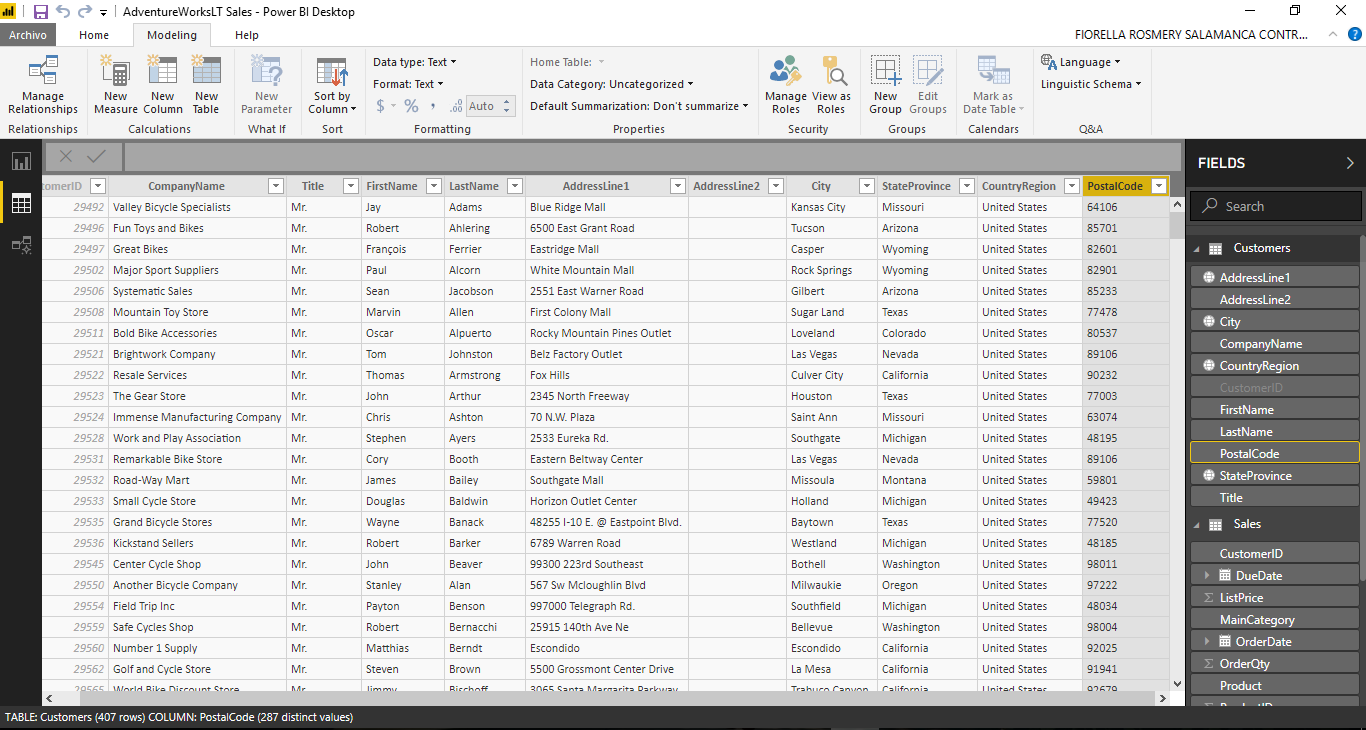
\includegraphics[width=17cm]{./Imagenes/Ejercicio1/Tarea3/17}
	\end{center}	

20. On the Modeling ribbon, in the Properties group, click Data Category: Uncategorized, and then click Postal Code.\\

	\begin{center}
	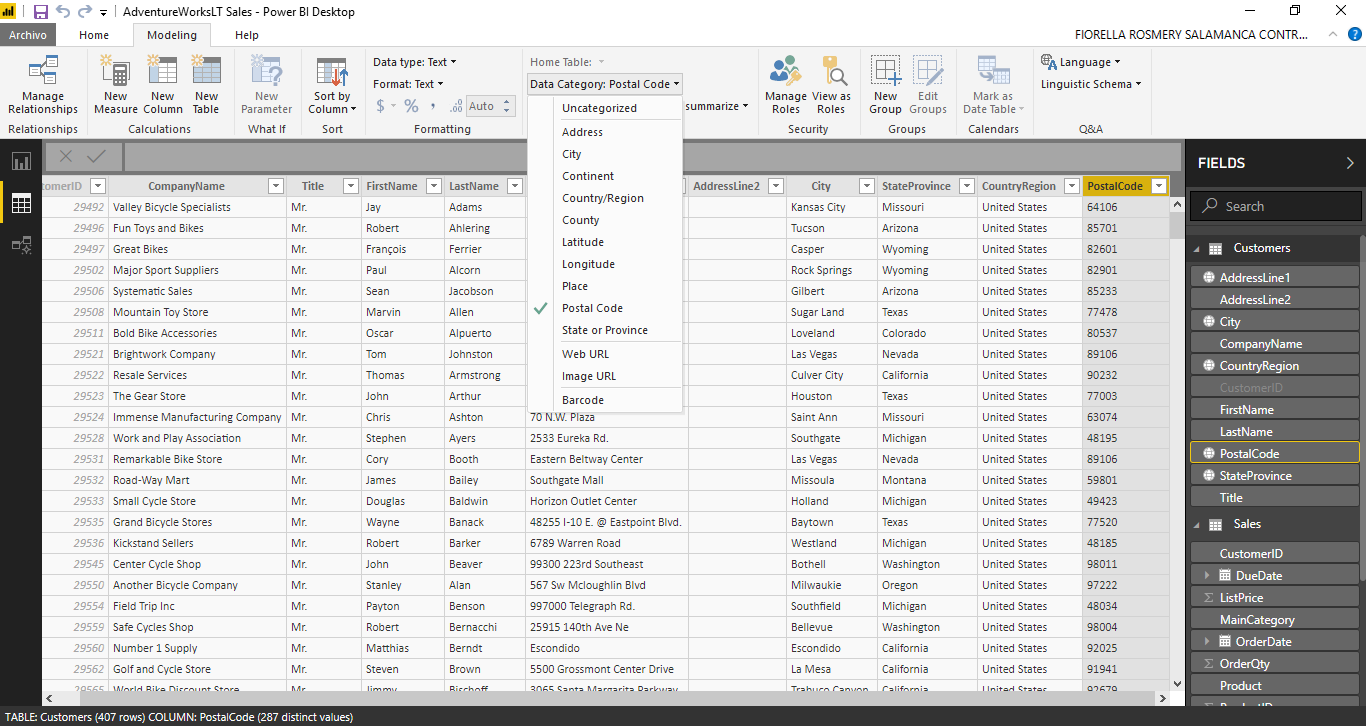
\includegraphics[width=17cm]{./Imagenes/Ejercicio1/Tarea3/18}
	\end{center}	

21. On the Modeling ribbon, in the Calculations group, click New Column, and then in the formula bar, type the following expression and press Enter:\\

\textbf{FullAddress = Customers[AddressLine1] \& ", " \& Customers[City] \& ", " \&
Customers[StateProvince] \& ", " \& Customers[CountryRegion] \& ", " \&
Customers[PostalCode]} 

	\begin{center}
	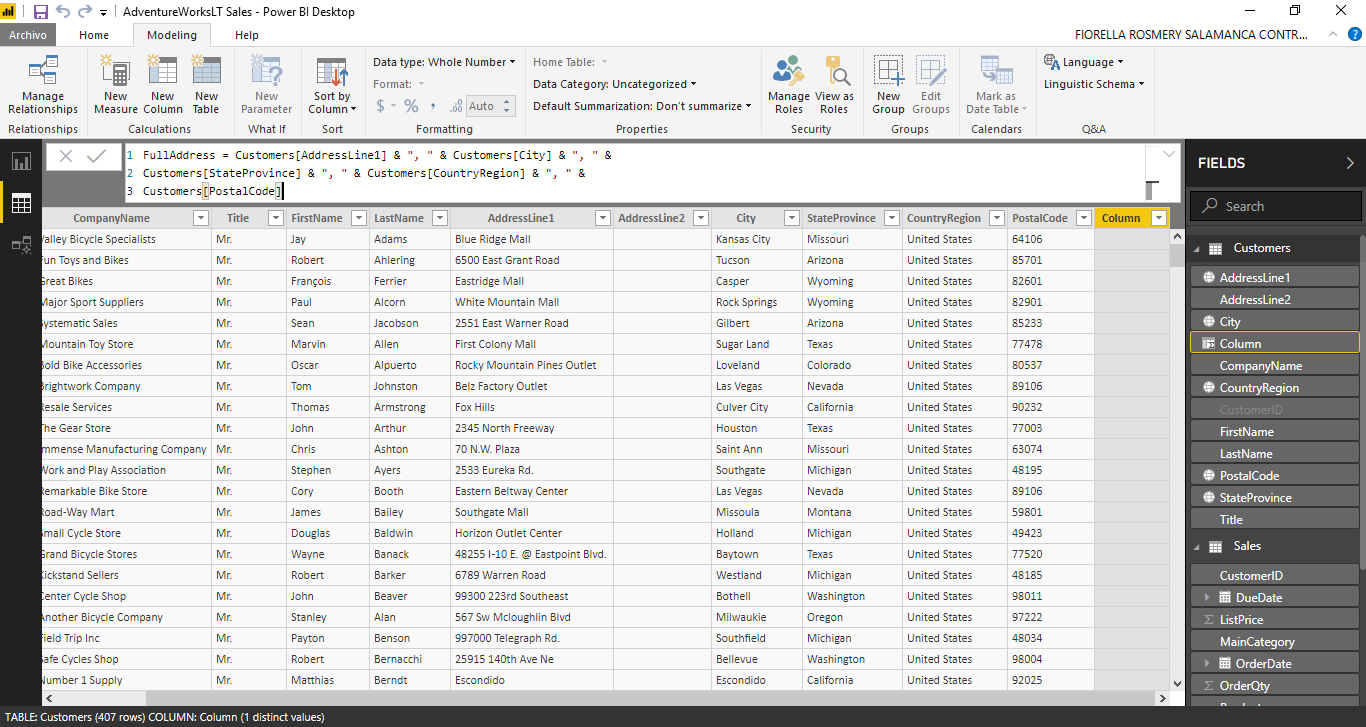
\includegraphics[width=17cm]{./Imagenes/Ejercicio1/Tarea3/19}
	\end{center}	

22. In the Fields pane, click Sales.\\

	\begin{center}
	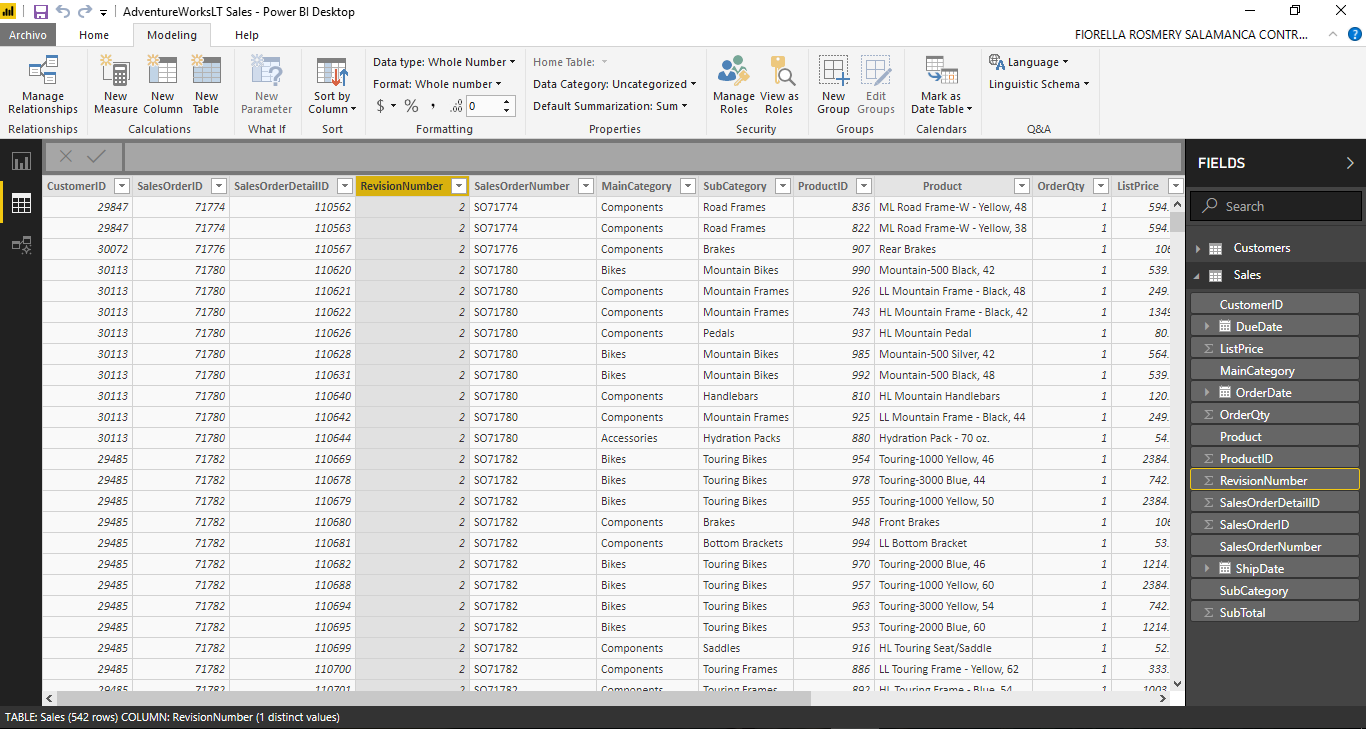
\includegraphics[width=17cm]{./Imagenes/Ejercicio1/Tarea3/20}
	\end{center}	

23. Right-click the RevisionNumber column, and click Delete.\\
24. In the Delete Column dialog box, click Delete.\\

	\begin{center}
	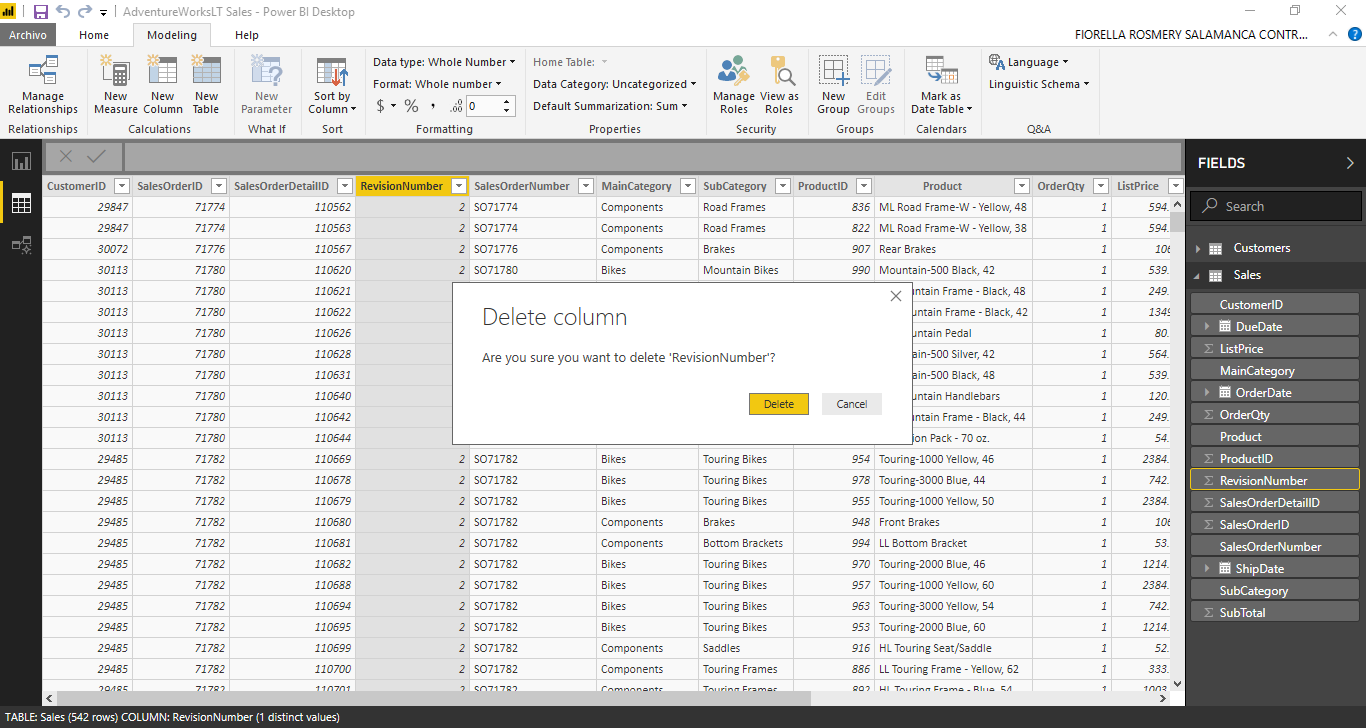
\includegraphics[width=17cm]{./Imagenes/Ejercicio1/Tarea3/21}
	\end{center}	

25. Right-click the SalesOrderNumber column, and click Delete.\\

	\begin{center}
	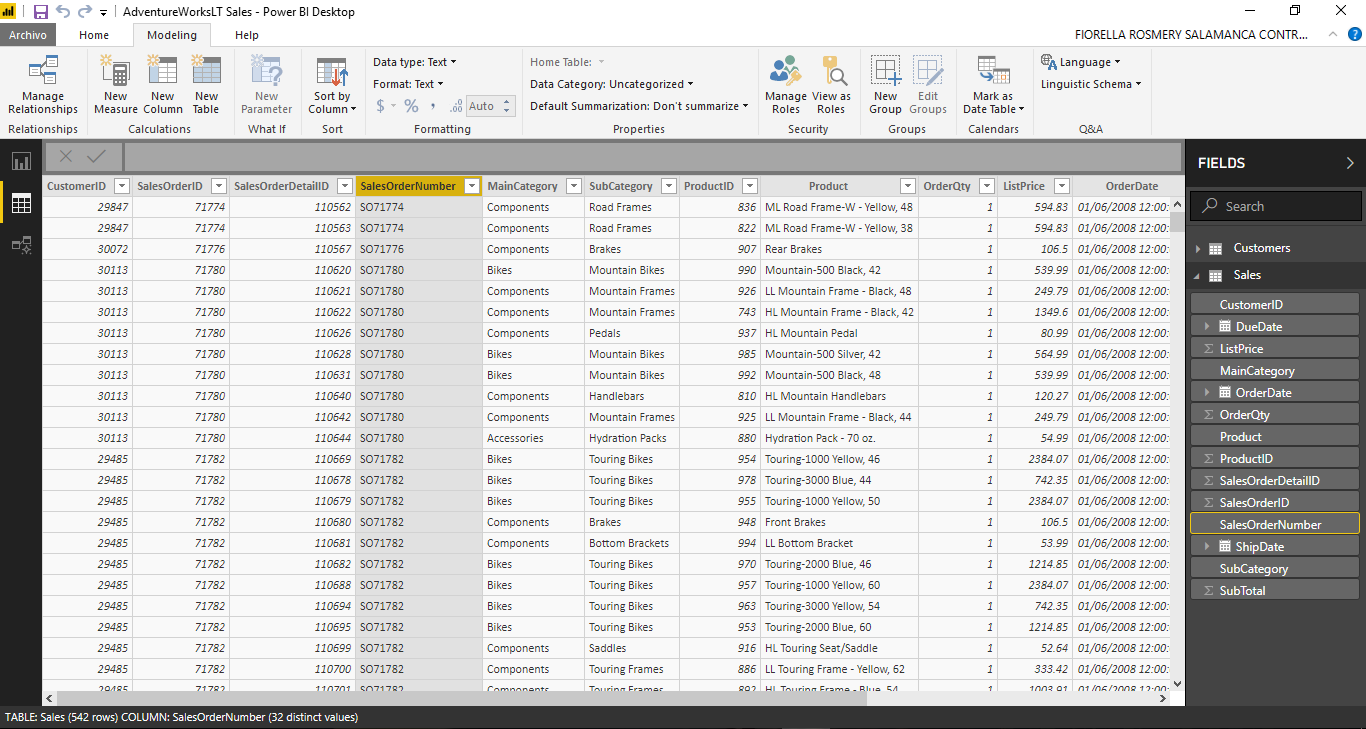
\includegraphics[width=17cm]{./Imagenes/Ejercicio1/Tarea3/22}
	\end{center}	

26. In the Delete Column dialog box, click Delete.\\

	\begin{center}
	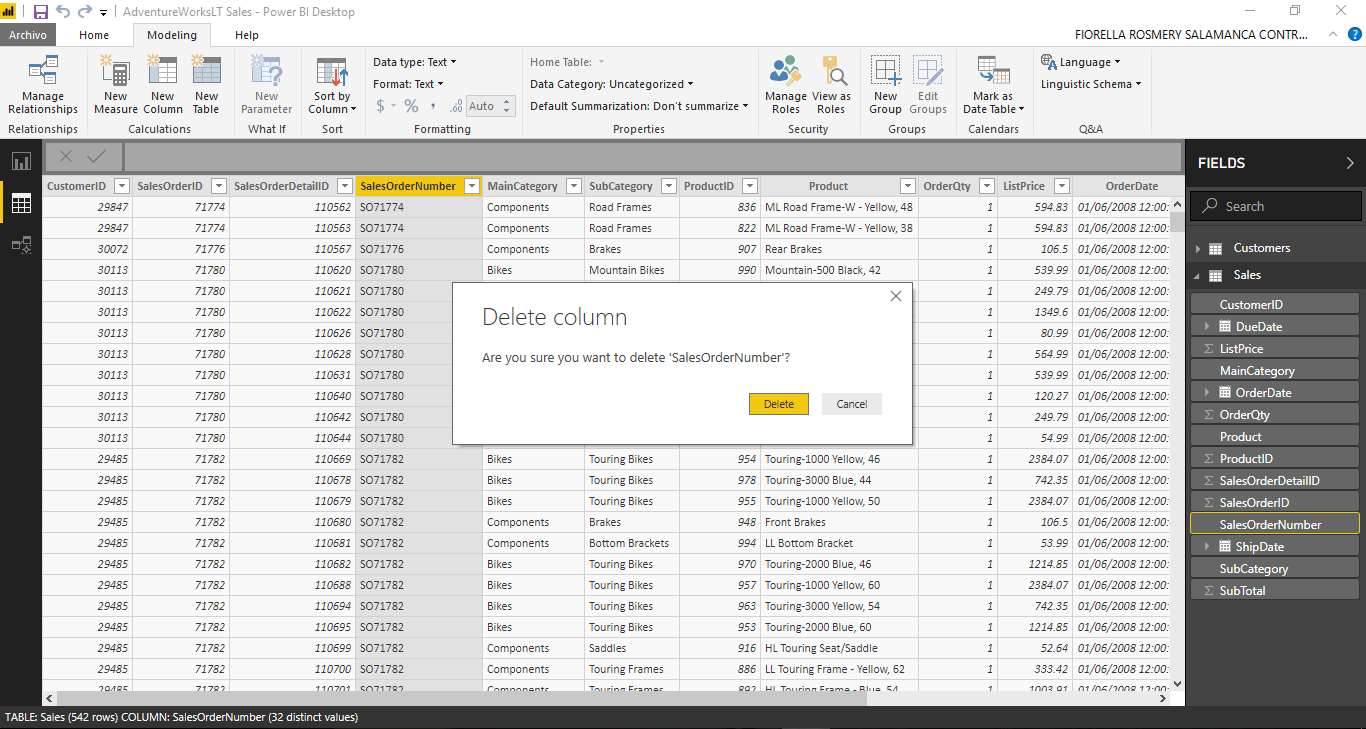
\includegraphics[width=17cm]{./Imagenes/Ejercicio1/Tarea3/23}
	\end{center}	

27. Right-click the CustomerID column, and then click Hide in Report View.\\

	\begin{center}
	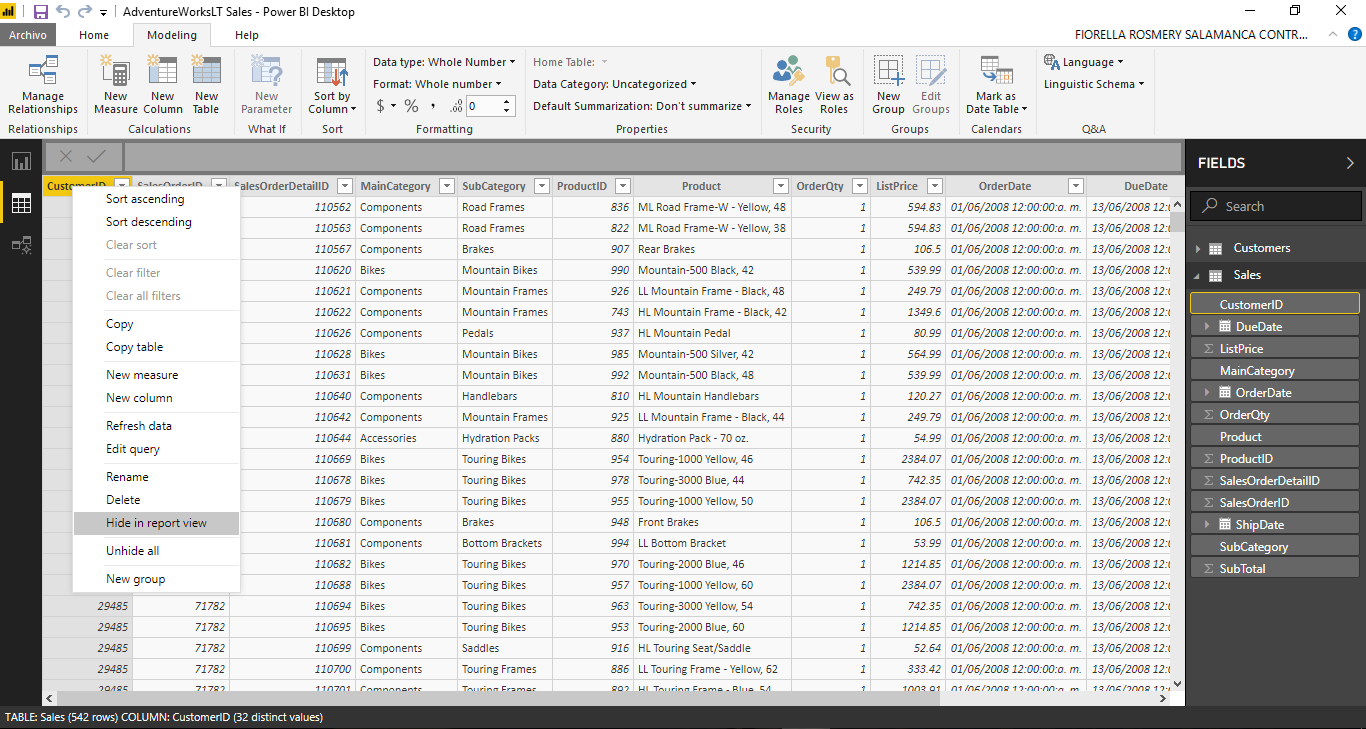
\includegraphics[width=17cm]{./Imagenes/Ejercicio1/Tarea3/24}
	\end{center}	

28. Right-click the SalesOrderID column, and then click Hide in Report View.\\

	\begin{center}
	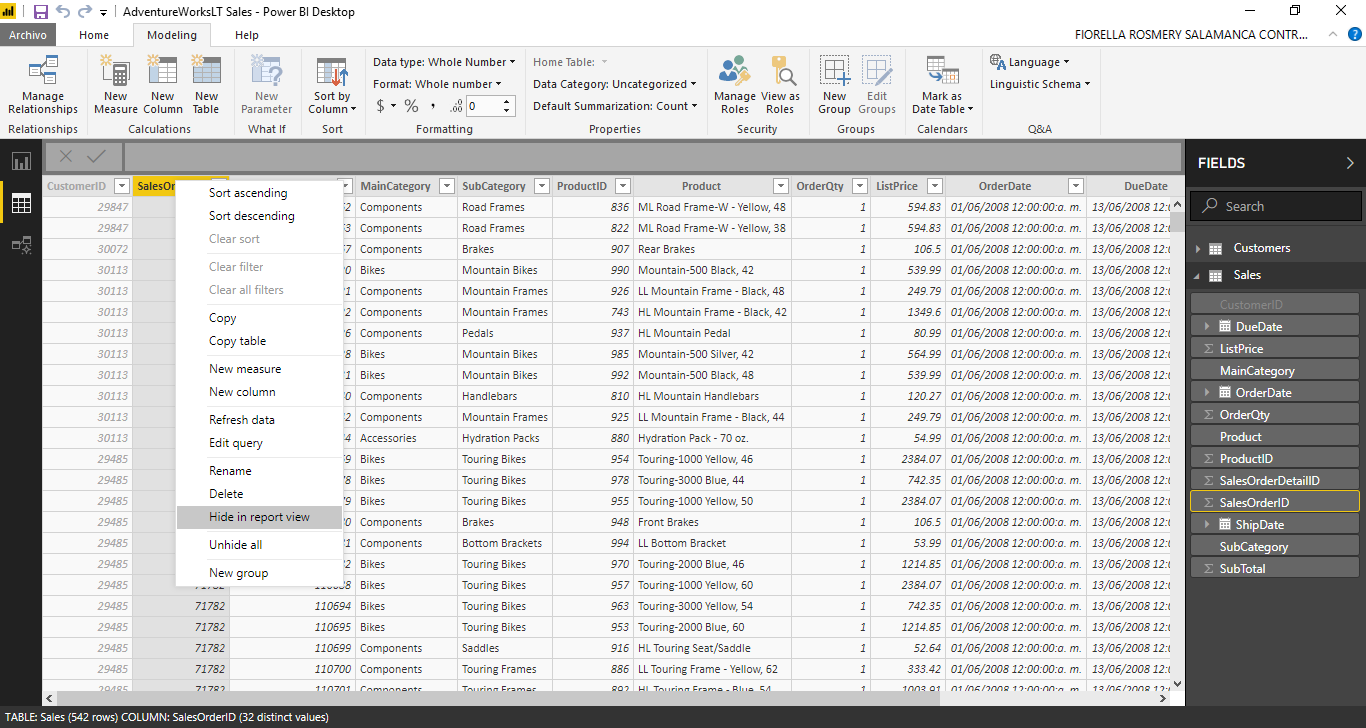
\includegraphics[width=17cm]{./Imagenes/Ejercicio1/Tarea3/25}
	\end{center}	

29. Right-click the SalesOrderDetailID column, and then click Hide in Report View.\\
30. On the Modeling ribbon, in the Calculations group, click New Column, and then in the formula bar, type the following expression and press Enter:\\

\textbf{LineTotal = Sales[OrderQty] * Sales[ListPrice]}

	\begin{center}
	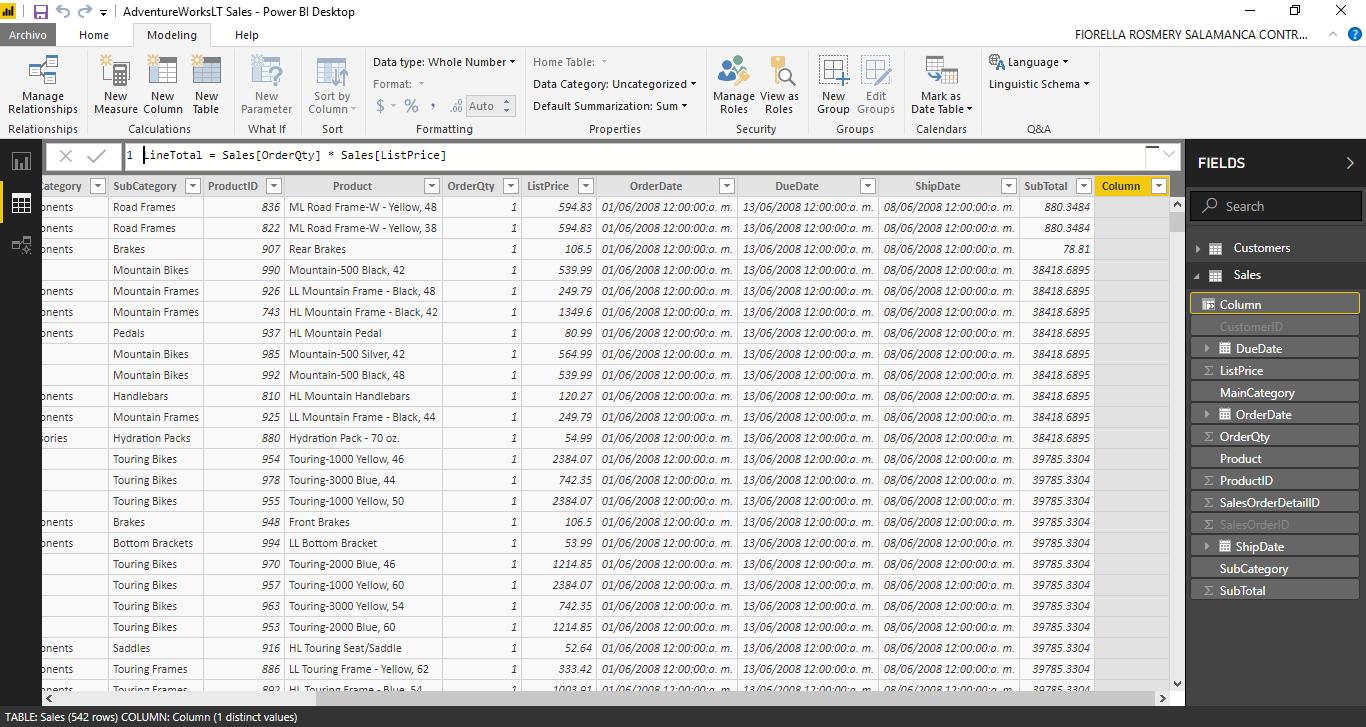
\includegraphics[width=17cm]{./Imagenes/Ejercicio1/Tarea3/26}
	\end{center}	

31. Click the LineTotal column header.\\
32. On the Modeling ribbon, in the Formatting group, click Format: General, point to Currency, and then click \$ English (United States).\\

	\begin{center}
	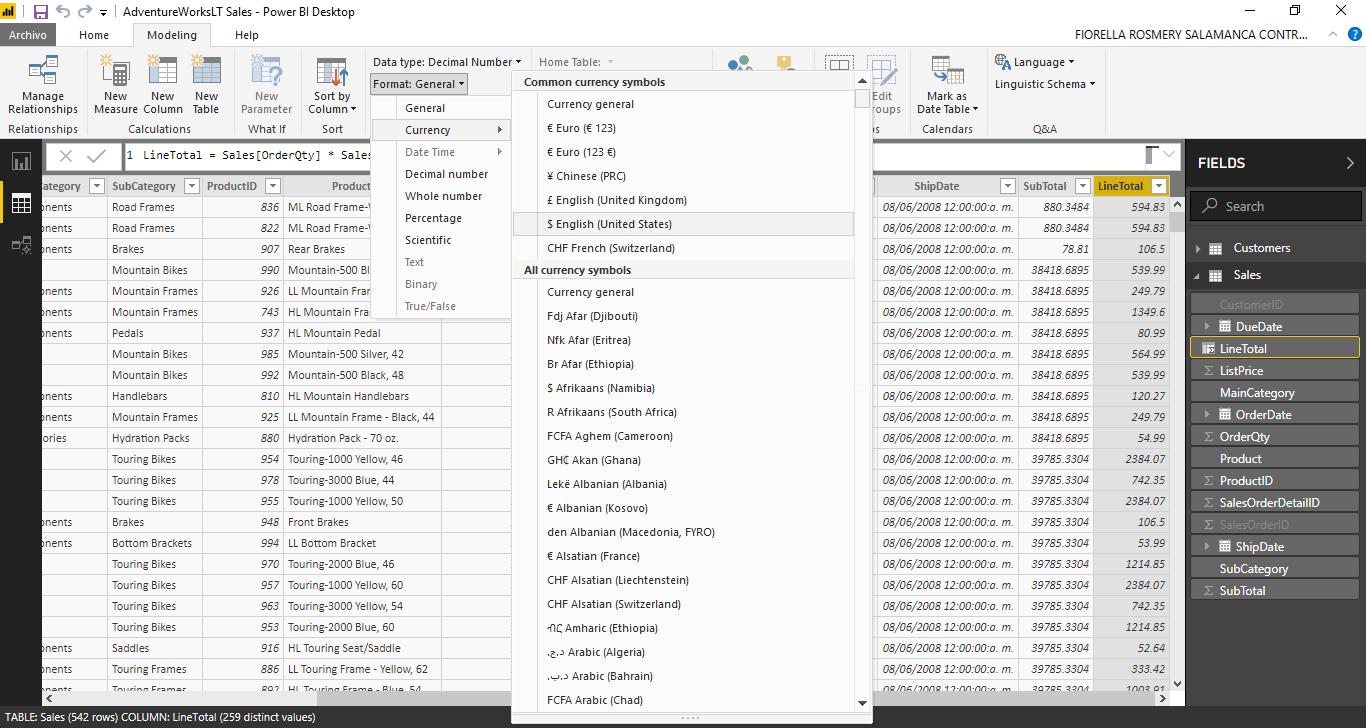
\includegraphics[width=17cm]{./Imagenes/Ejercicio1/Tarea3/27}
	\end{center}	

33. On the Modeling ribbon, in the Calculations group, click New Measure, and then in the formula bar, type the following expression and press Enter:\\

\textbf{TargetSales = SUM('Sales'[LineTotal]) * 1.2}

	\begin{center}
	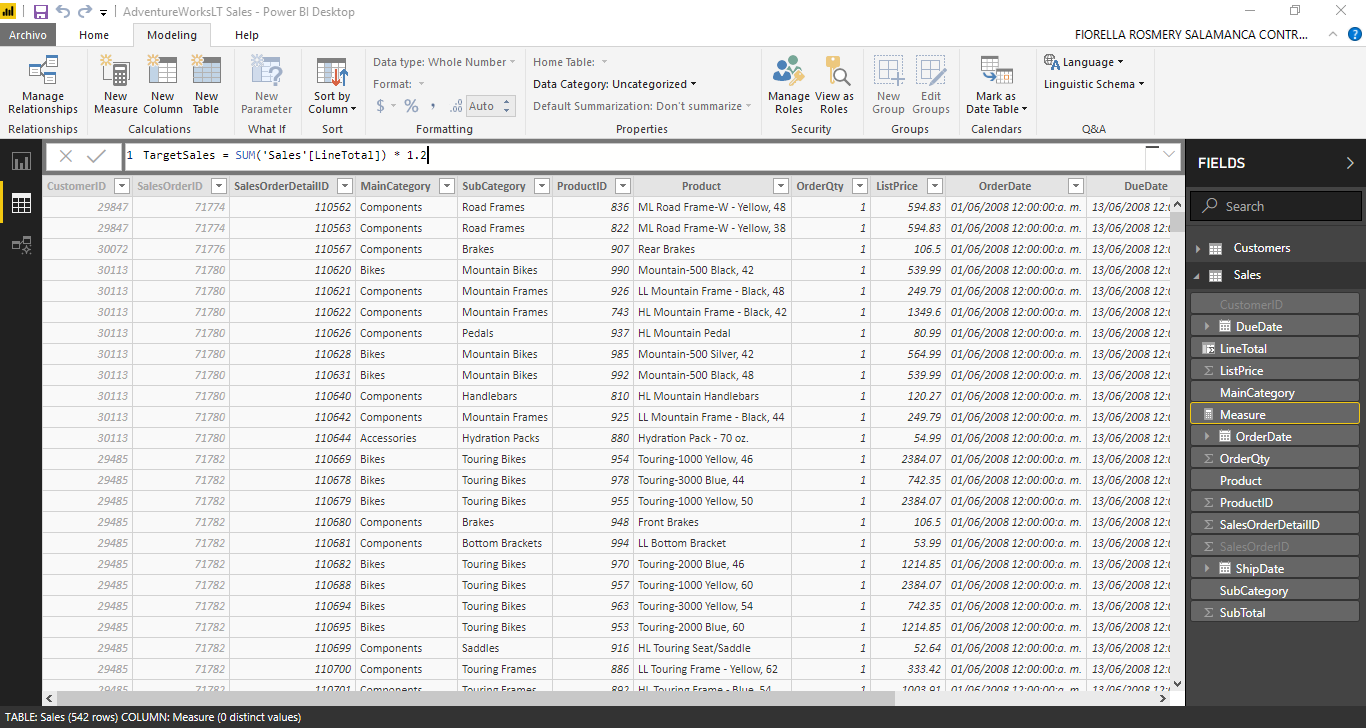
\includegraphics[width=17cm]{./Imagenes/Ejercicio1/Tarea3/29}
	\end{center}	

34. Click Save, and then leave Power BI Desktop open for the next task.

\section{Ejercicio 1: Conexión a datos de Power BI - Tarea 4: Combinar datos} 

1. In File Explorer, browse to the D:/Labfiles/Lab06/Starter/Project folder, and then open the
States.xlsx file.\\

	\begin{center}
	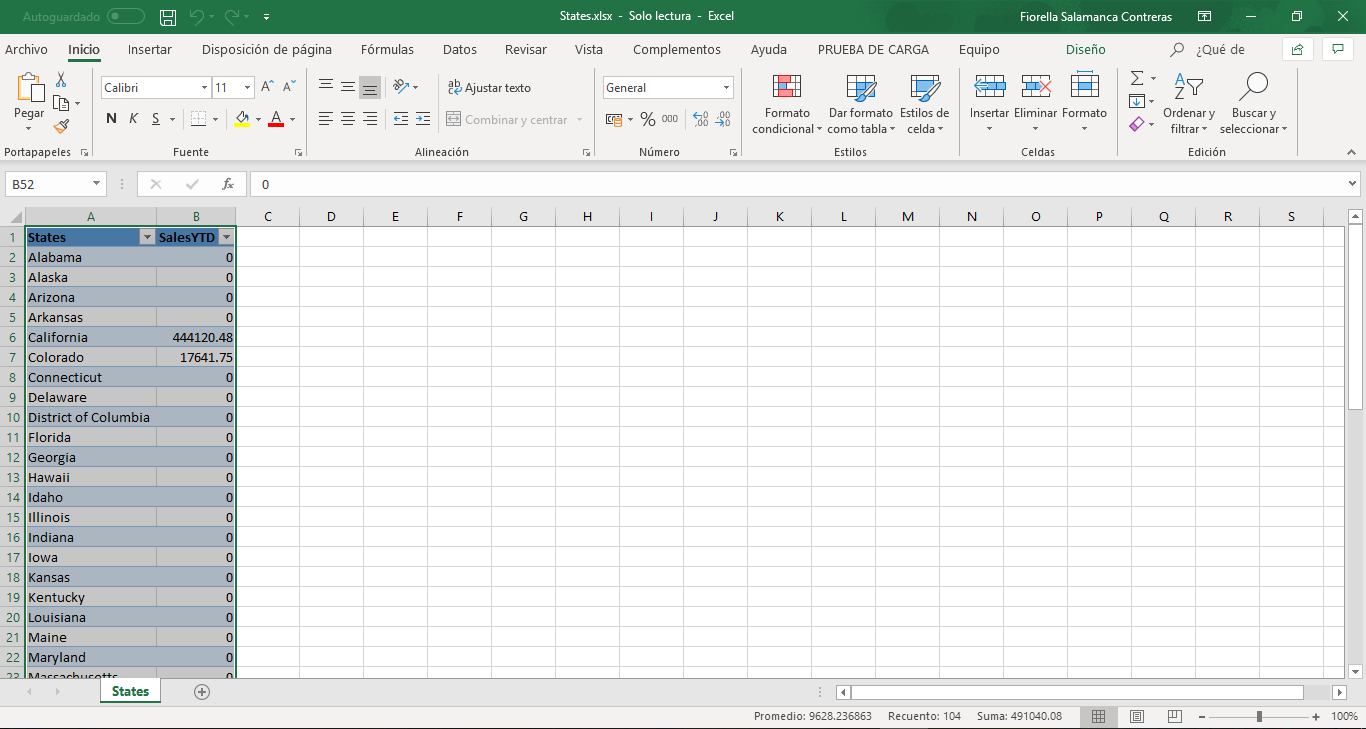
\includegraphics[width=17cm]{./Imagenes/Ejercicio1/Tarea4/1}
	\end{center}	

2. In the States worksheet, select all of the values in the two columns, and then press Ctrl+C.\\
3. In Power BI Desktop, on the Home ribbon, click Enter Data.\\

	\begin{center}
	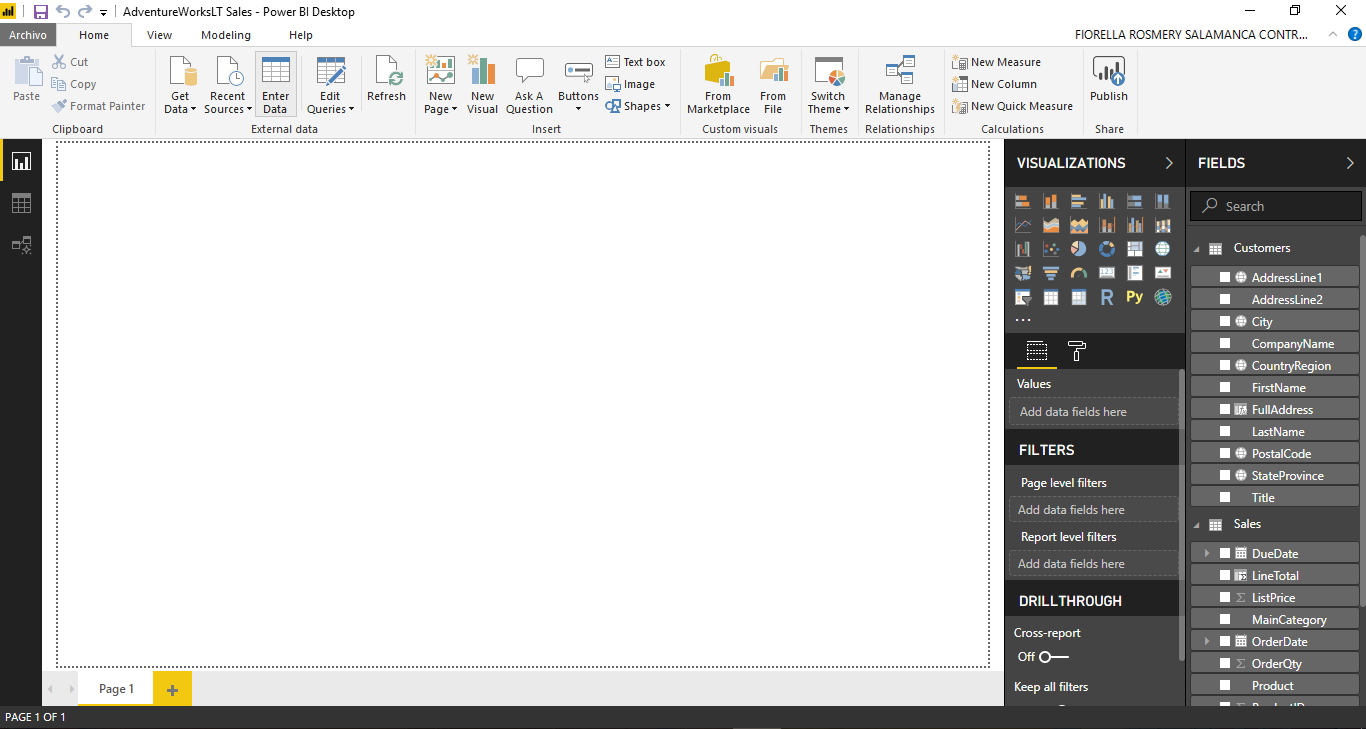
\includegraphics[width=17cm]{./Imagenes/Ejercicio1/Tarea4/2}
	\end{center}	

4. In the Create Table dialog box, click in the table, and then press Ctrl+V. Power BI detects that the first row is a column header.\\
5. In the Name box, type Sales by State, and then click Load.\\

	\begin{center}
	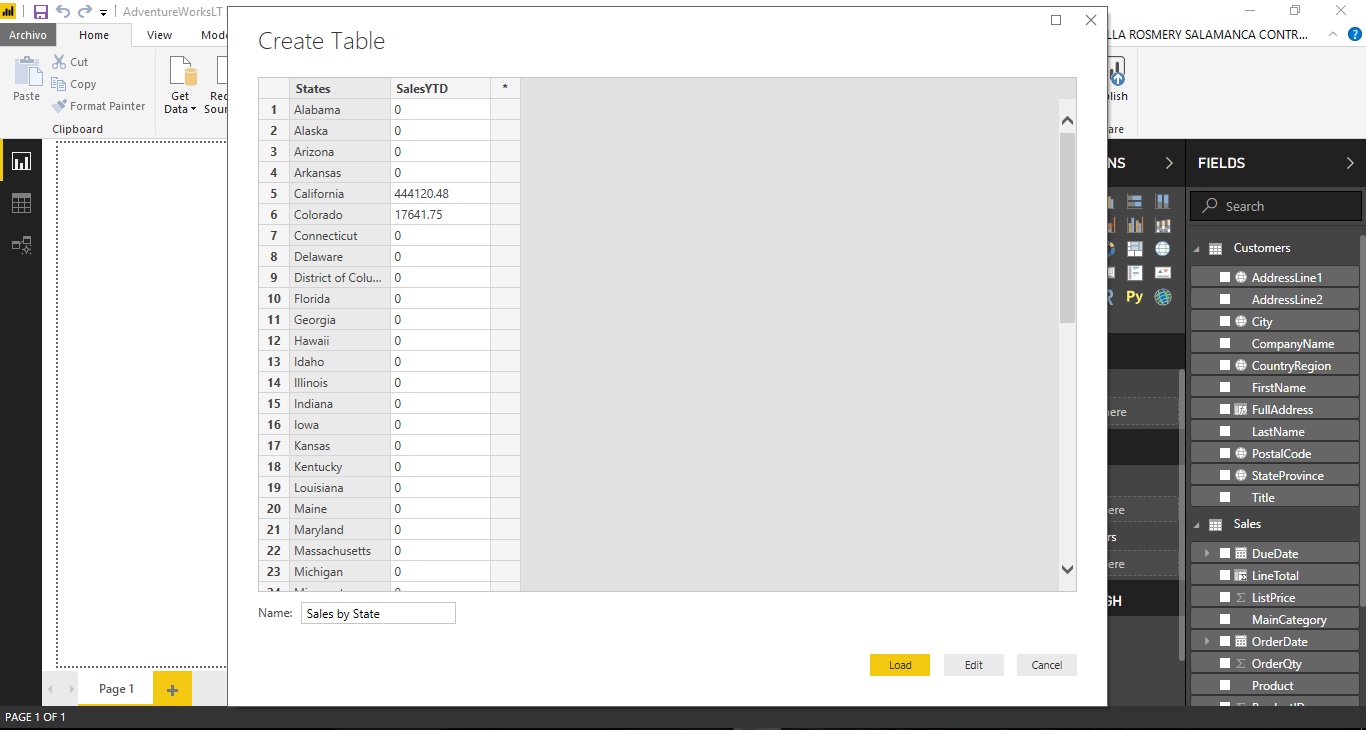
\includegraphics[width=17cm]{./Imagenes/Ejercicio1/Tarea4/3}
	\end{center}	

6. On the Home ribbon, click Get Data, and then click Web.\\

	\begin{center}
	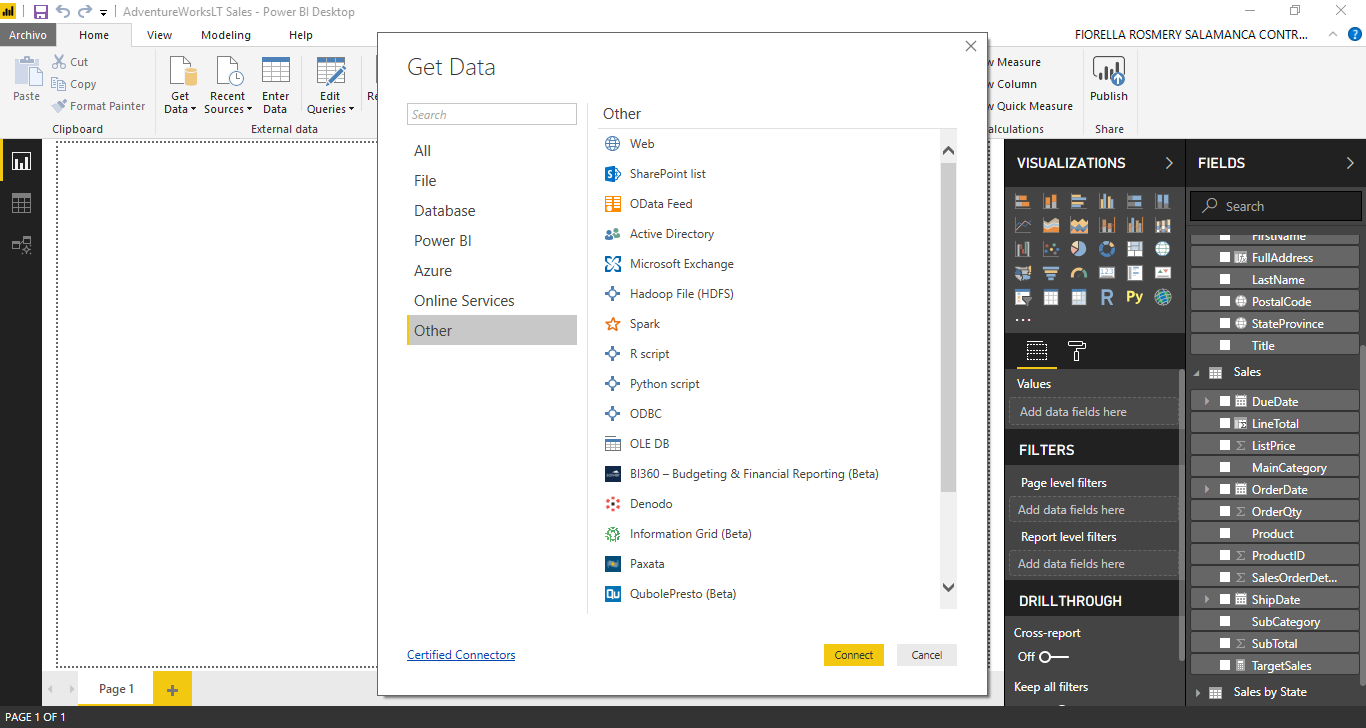
\includegraphics[width=17cm]{./Imagenes/Ejercicio1/Tarea4/4}
	\end{center}	


7. In the From Web dialog box, in the URL box, type http://en.wikipedia.org/wiki/List\_of\_U.S.\_state\_abbreviations, and then click OK.\\

	\begin{center}
	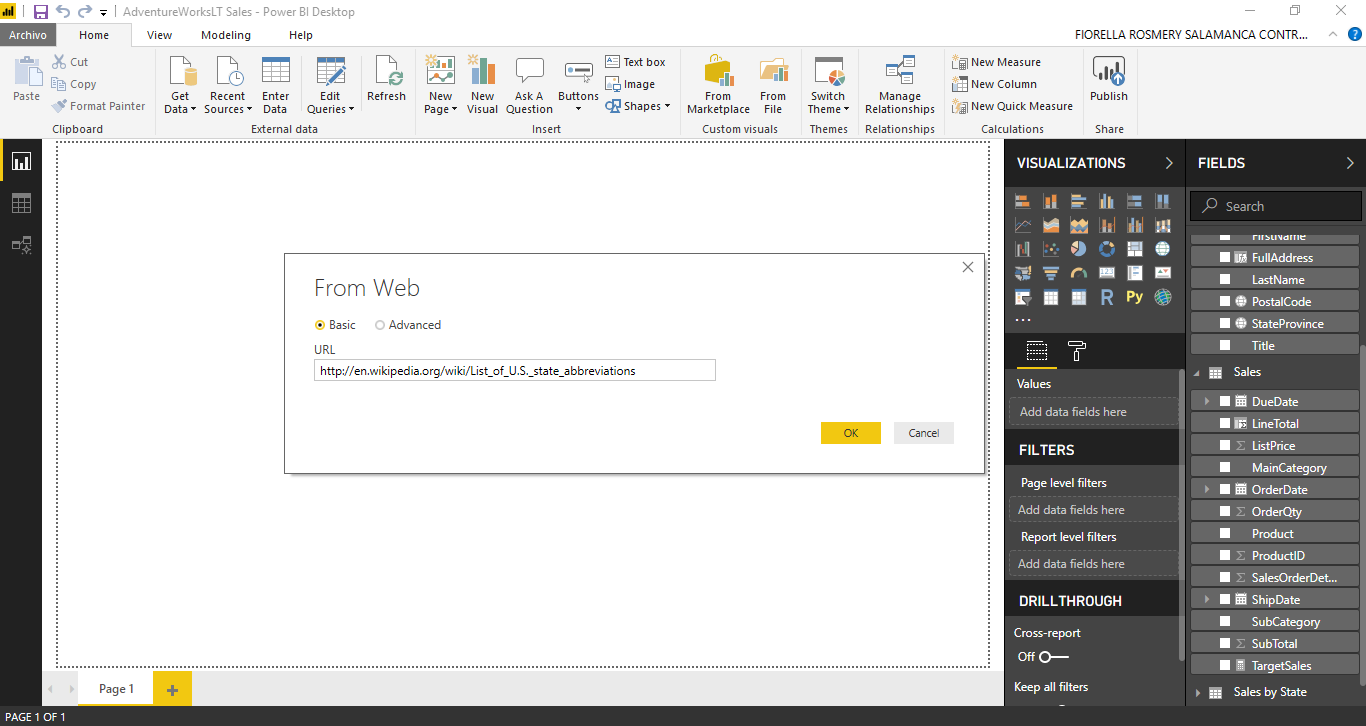
\includegraphics[width=17cm]{./Imagenes/Ejercicio1/Tarea4/5}
	\end{center}	

8. In the Navigator dialog box, select Codes and abbreviations for U.S. states, territories and other regions, and then click Load.\\

	\begin{center}
	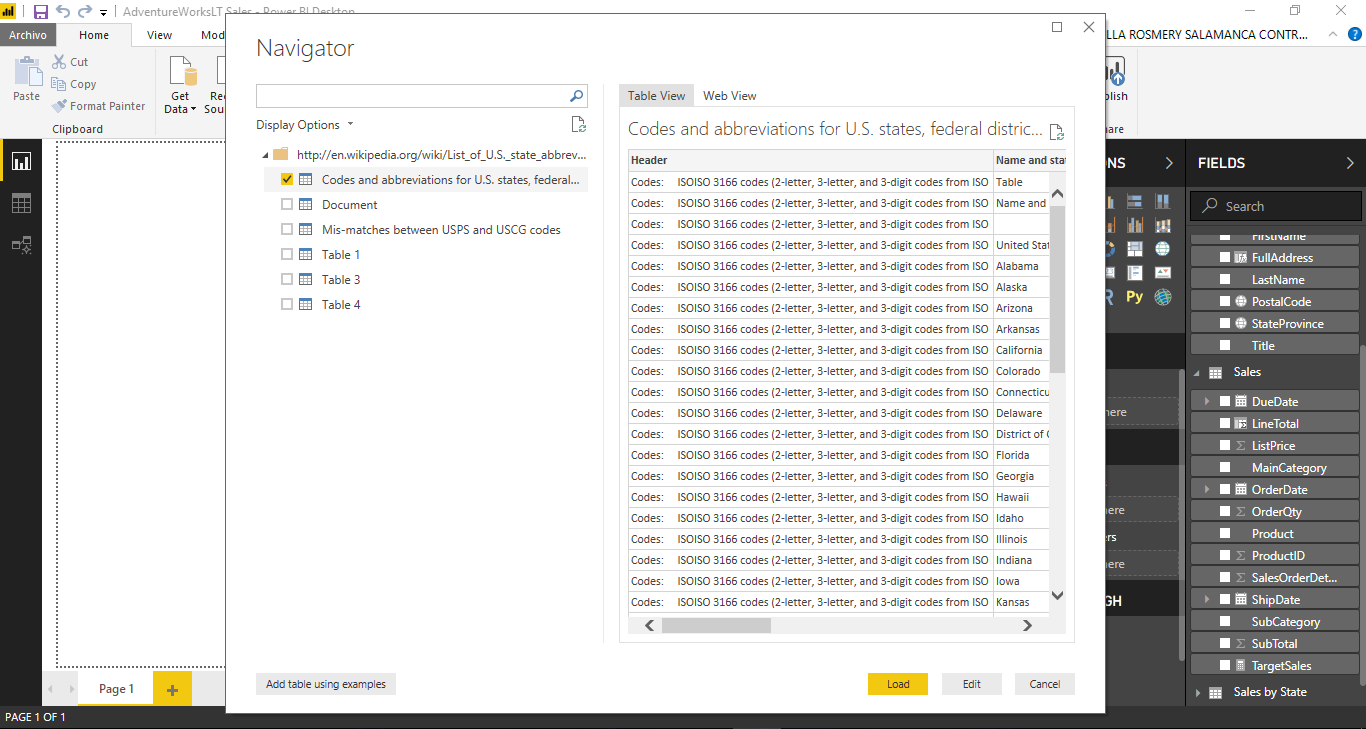
\includegraphics[width=17cm]{./Imagenes/Ejercicio1/Tarea4/6}
	\end{center}	

9. In the Fields pane, click Codes and abbreviations for U.S. states, territories and other regions to display the data. The table has 26 rows at the bottom that are not needed.\\

	\begin{center}
	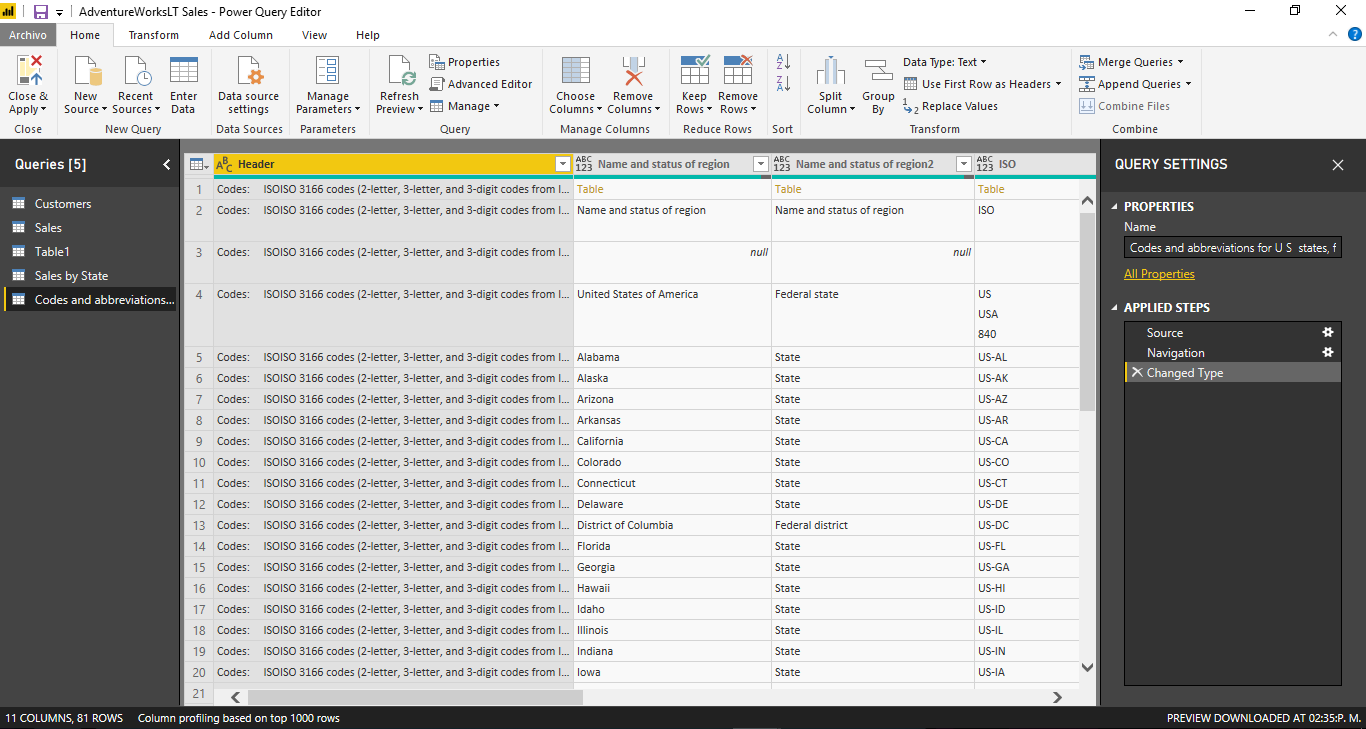
\includegraphics[width=17cm]{./Imagenes/Ejercicio1/Tarea4/7}
	\end{center}	

10. On the Home ribbon, in the External Data group, click Edit Queries, then click Edit Queries.\\
11. In Query Editor, in the Queries pane, click Codes and abbreviations for U.S. states, territories and
other regions.\\
12. On the Home ribbon, click Reduce Rows, click Remove Rows, and then click Remove Bottom
Rows.\\

	\begin{center}
	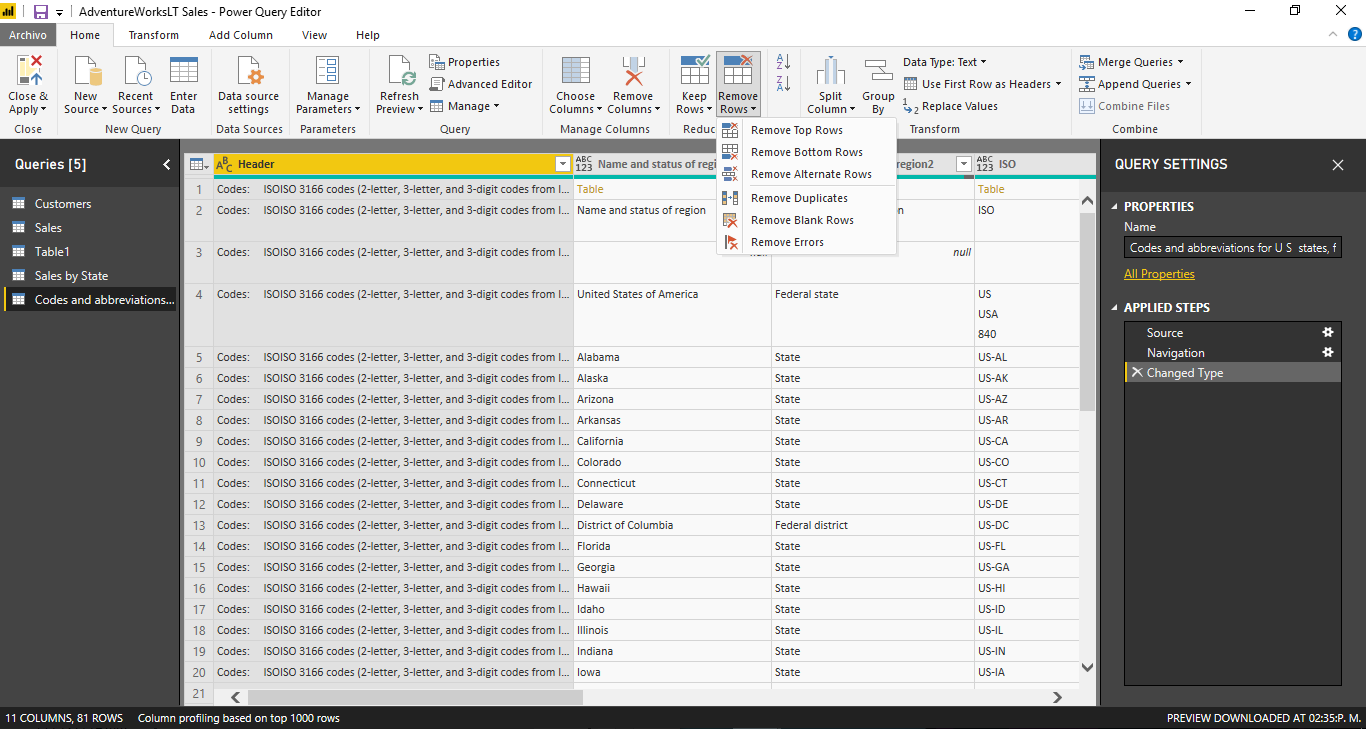
\includegraphics[width=17cm]{./Imagenes/Ejercicio1/Tarea4/8}
	\end{center}	

13. In the Remove Bottom Rows dialog box, in the Number of rows box, type 26, and then click OK.\\

	\begin{center}
	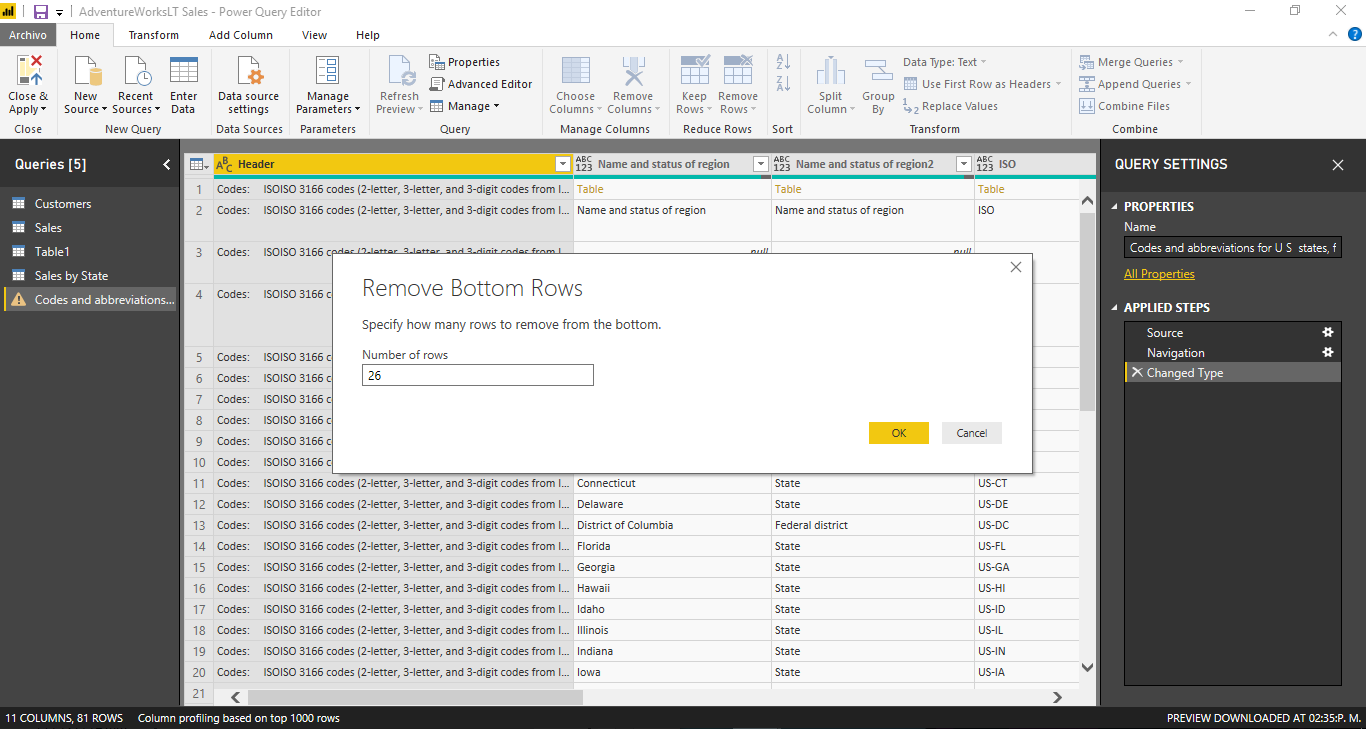
\includegraphics[width=17cm]{./Imagenes/Ejercicio1/Tarea4/9}
	\end{center}	

14. Click the ANSI2 column header, and then hold down the Ctrl key while selecting all of the columns to
the right. This selects multiple rows.\\

	\begin{center}
	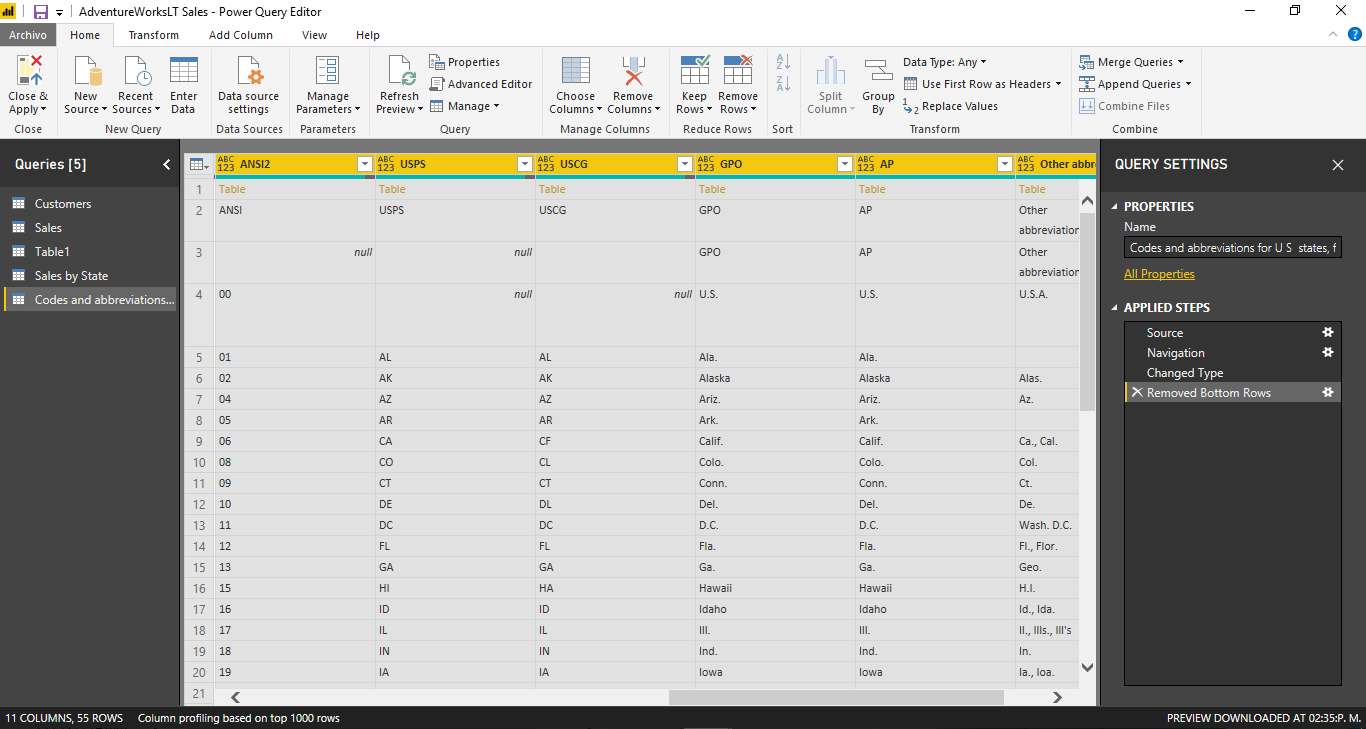
\includegraphics[width=17cm]{./Imagenes/Ejercicio1/Tarea4/10}
	\end{center}	

15. Still holding down Ctrl, click the Name and status of region2 and Header columns to include this in
the selection.\\

	\begin{center}
	\includegraphics[width=17cm]{./Imagenes/Ejercicio1/Tarea4/11}
	\end{center}	

16. On the Home ribbon, click Manage Columns, click Remove Columns, and then click Remove Columns.\\
17. In the Query Settings pane, under Properties, in the Name box, type States with Codes, and then
press Enter.\\

	\begin{center}
	\includegraphics[width=17cm]{./Imagenes/Ejercicio1/Tarea4/12}
	\end{center}	

18. On the Home ribbon, in the Transform group, click Use First Row as Headers.\\
19. Right-click the United States of America column header, click Rename, type State Name, and then
press Enter.\\

	\begin{center}
	\includegraphics[width=17cm]{./Imagenes/Ejercicio1/Tarea4/13}
	\end{center}	

20. Right-click the US USA 840 column header, click Rename, type State Code Long, and then press
Enter.\\

	\begin{center}
	\includegraphics[width=17cm]{./Imagenes/Ejercicio1/Tarea4/14}
	\end{center}	

21. Right-click the US column header, click Rename, type State Code Short, and then press Enter.\\

	\begin{center}
	\includegraphics[width=17cm]{./Imagenes/Ejercicio1/Tarea4/16}
	\end{center}	

22. In the Queries pane, click Sales by State.\\
23. On the Home ribbon, click Combine, and then click Merge Queries.\\
24. In the Merge dialog box, in the Sales by State table, click the States column.\\
25. In the list, click States with Codes, click the State Name column, and then click OK. The new column
is added to the table and contains the merged States with Codes table.\\

	\begin{center}
	\includegraphics[width=17cm]{./Imagenes/Ejercicio1/Tarea4/16}
	\end{center}	

26. In the column header, click the Expand icon, clear (Select All Columns), select State Code Short,
and then click OK. The column now shows just the state codes.\\

	\begin{center}
	\includegraphics[width=17cm]{./Imagenes/Ejercicio1/Tarea4/17}
	\end{center}	

27. Right-click the column, click Rename, type State Code, and then press Enter.\\
28. On the File menu, click Close \& Apply.\\

	\begin{center}
	\includegraphics[width=17cm]{./Imagenes/Ejercicio1/Tarea4/18}
	\end{center}	

29. In the Fields pane, right-click States with Codes, and then click Hide in Report View.\\

	\begin{center}
	\includegraphics[width=17cm]{./Imagenes/Ejercicio1/Tarea4/19}
	\end{center}	

Results: After this exercise, you should have imported data from Azure, shaped it by using the Power BI
transformation tools, and combined the data by merging columns and appending rows.\\
\section{Ejercicio 2: Construyendo Reportes en Power BI - Tarea 1: Crear un Grafico} 

1. En Power BI Desktop, en la barra derecha de navegación, hacer click en Reporte (Report).\\
2. En el panel de Visualizaciones (Visualizations), hacer click en Gauge.\\
3. Arrastar el campo (LineTotal) de la table (Sales) a la propiedad Valor (Value) del objeto gauge.\\
4. Arrastrar la medida Drag the TargetSales measure from the Sales table to the Target value property of the
gauge.\\
5. Click Format, expand Gauge axis, and then in the Max box, type 146000.\\
6. Expand Title, in the Title Text box, type Target Sales, and then click Center.\\

	\begin{center}
	\includegraphics[width=17cm]{./Imagenes/Ejercicio2/Tarea1/1}
	\end{center}	

7. Click the report canvas, and then drag the CompanyName field from the Customers table onto the
report. Power BI automatically creates a table.\\
8. Drag the LineTotal field from the Sales table onto the report.\\
9. Make sure that the table has focus, and then in the Visualizations pane, click Pie chart.\\
10. Expand the chart to make all of the company names visible by using the resizer handles on the edge
of the chart.\\
11. With the focus still on the pie chart, click Format, and then expand Title.\\
12. In the Title Text box, type Top Selling Customers, and then click Center.\\

	\begin{center}
	\includegraphics[width=17cm]{./Imagenes/Ejercicio2/Tarea1/2}
	\end{center}	

13. Drag the MainCategory field from the Sales table onto the report canvas. Power BI creates a table.\\
14. Drag the OrderQty field onto the table.\\
15. In the Visualizations pane, click Stacked bar chart.\\
16. In the Visualizations pane, click Fields.\\
17. Drag the OrderQty field onto the Color saturation property. Notice that the colors change.\\
18. In the Visualizations pane, click Analytics, expand Constant Line, and then click Add.\\
19. In the Value box, type 500.\\
20. Change Color to red, toggle Data label to On, and then change the color to red.\\
21. In the Visualizations pane, click Format, and expand Title.\\
22. In the Title Text box, type Orders by Main Category, and then click Center.\\

	\begin{center}
	\includegraphics[width=17cm]{./Imagenes/Ejercicio2/Tarea1/3}
	\end{center}	

23. Click the report canvas to give it focus, and then in the Visualizations pane, click Donut chart.\\
24. In the Sales table, select MainCategory and LineTotal.\\
25. In the Visualizations pane, click Format, and then expand Title.\\
26. In the Title Text box, type Sales by Main Category, and then click Center.\\

	\begin{center}
	\includegraphics[width=17cm]{./Imagenes/Ejercicio2/Tarea1/4}
	\end{center}	

27. Drag the Product field from the Sales table onto the report canvas. Power BI creates a table.\\
28. Drag the LineTotal field from the Sales table onto the products table chart.\\
29. In the Sales table, select the MainCategory field.\\
30. In the Visualizations pane, click Fields.\\
31. In the Filters pane, expand LineTotal(All).\\
32. In the Show items when the value list, select is greater than, and then in the box below, type
32000.\\
33. Click Apply filter.\\
34. Expand MainCategory(All), and then select Bikes.\\
35. In the Visualizations pane, click Stacked column chart.\\
36. In the Visualizations pane, click Format, and then expand Title.\\
37. In the Title Text box, type Top 10 Selling Bikes, and then click Center.\\

	\begin{center}
	\includegraphics[width=17cm]{./Imagenes/Ejercicio2/Tarea1/5}
	\end{center}	

38. In the Visualizations pane, click Analytics, expand Constant Line, and then click Add.\\
39. In the Value box, type 35000, and then set Color to red.\\
40. Toggle Data label to On, and then set Color to red.\\
41. Expand the chart to fill the remaining space on the report canvas. If necessary, move your visuals
around to make them fit.\\
42. Click Save.\\
\section{Ejercicio 2: Construyendo Reportes en Power BI - Tarea 2: Crear una Visualización de Mapa a Map Visualization} 

1. At the bottom of the report, click the + icon to add a new page.\\
2. In the Fields pane, in the Customers table, select the City field. Power BI adds a map to the report.\\
3. In the Fields pane, in the Sales table, select the LineTotal field.\\
4. Using the grabber tool on the right side of the chart, resize the map to show all of the bubbles.\\
5. Notice that the bubbles are proportionally sized to represent the data.\\
6. In the Visualizations pane, click Format, and then expand Title.\\
7. In the Title Text box, type World Sales by City, and then click Center.\\

	\begin{center}
	\includegraphics[width=17cm]{./Imagenes/Ejercicio2/Tarea2/1}
	\end{center}	

8. Click the report canvas, and then in the Sales by State table, select the State Code column. Power BI
automatically adds a map.\\
9. In the Sales by State table, select the SalesYTD column.\\
10. In the Visualizations pane, click Filled Map. Using the grabber tool on the right side and at the
bottom of the chart, resize the map to show all the states.\\
11. Notice that the sales cluster in one area.\\
12. Position the cursor on California(CA) to see the sales figure. The value has not been formatted as
currency.\\
13. In the Sales by State table, click the SalesYTD column.\\
14. On the Modeling ribbon, select Format:General, click Currency, and then select \$ English (United
Stated).\\
15. Position the cursor on California(CA) on the map, and notice that the value has been formatted.\\
16. In the Visualizations pane, click Format, and then expand Title.\\
17. In the Title Text box, type Sales by State, and then click Center.\\

	\begin{center}
	\includegraphics[width=17cm]{./Imagenes/Ejercicio2/Tarea2/2}
	\end{center}	

18. Click Save, and then leave the report open for the next exercise.\\
Results: After this exercise, you should have created a report that has chart visuals and is ready to publish to the Power BI service.
\section{Ejercicio 3: Crear un panel de Power BI - Tarea 1: Publicar Informes desde Power BI Desktop} 

1. On the Home ribbon, click Publish.\\
2. In the Sign in to your account dialog box, enter your username (email address) and password, and
then click Sign in.\\
3. In the Publishing to Power BI dialog box, when the Success label shows, click Open
'AdventureWorksLT Sales.pbix' in Power BI.\\

	\begin{center}
	\includegraphics[width=13cm]{./Imagenes/Ejercicio3/Tarea1/1}
	\end{center}	

4. Internet Explorer will open. If prompted to sign in, enter your username (email address) and
password, and then click Sign in.\\
5. The report is loaded into the Power BI service.\\

	\begin{center}
	\includegraphics[width=15cm]{./Imagenes/Ejercicio3/Tarea1/2}
	\end{center}	

6. Remain signed in for the next task.\\
\section{Ejercicio 3: Crear un panel de Power BI - Tarea 2: Crear un Panel de Power BI} 

1. In Power BI, in the top-left corner, click Show the navigation pane.\\
2. Under Reports, click AdventureWorksLT Sales.\\
3. At the bottom of the page, click Page 1, click the Target Sales visual, and then click Pin visual.\\

	\begin{center}
	\includegraphics[width=17cm]{./Imagenes/Ejercicio3/Tarea2/1}
	\end{center}	

4. In the Pin to dashboard dialog box, click New dashboard, type AdventureWorksLT Sales, and
then click Pin.\\

	\begin{center}
	\includegraphics[width=17cm]{./Imagenes/Ejercicio3/Tarea2/2}
	\end{center}	

5. On the Top Selling Customers visual, click Pin visual.\\

	\begin{center}
	\includegraphics[width=17cm]{./Imagenes/Ejercicio3/Tarea2/3}
	\end{center}	

6. In the Pin to dashboard dialog box, click Existing dashboard, in the list, click AdventureWorksLT
Sales, and then click Pin.\\

	\begin{center}
	\includegraphics[width=17cm]{./Imagenes/Ejercicio3/Tarea2/4}
	\end{center}	

7. On the Orders by Main Category visual, click Pin visual.\\

	\begin{center}
	\includegraphics[width=17cm]{./Imagenes/Ejercicio3/Tarea2/5}
	\end{center}	

8. In the Pin to dashboard dialog box, click Existing dashboard, in the list, click AdventureWorksLT
Sales, and then click Pin.\\

	\begin{center}
	\includegraphics[width=17cm]{./Imagenes/Ejercicio3/Tarea2/6}
	\end{center}	

9. On the Top 10 Selling Bikes visual, click Pin visual.\\

	\begin{center}
	\includegraphics[width=17cm]{./Imagenes/Ejercicio3/Tarea2/7}
	\end{center}	

10. In the Pin to dashboard dialog box, click Existing dashboard, in the list, click AdventureWorksLT
Sales, and then click Pin.\\

	\begin{center}
	\includegraphics[width=17cm]{./Imagenes/Ejercicio3/Tarea2/8}
	\end{center}	

11. On the Sales by Main Category visual, click Pin visual.\\

	\begin{center}
	\includegraphics[width=17cm]{./Imagenes/Ejercicio3/Tarea2/9}
	\end{center}	

12. In the Pin to dashboard dialog box, click Existing dashboard, in the list, click AdventureWorksLT
Sales, and then click Pin.\\

	\begin{center}
	\includegraphics[width=17cm]{./Imagenes/Ejercicio3/Tarea2/10}
	\end{center}	

13. The dashboard is listed in the My Workspace pane, under Dashboards. Notice the yellow star icon
to denote that this is a new dashboard.\\
14. Click the AdventureWorksLT Sales dashboard to open it.\\
15. Notice that the tiles are all the same size.\\
16. On the Target Sales tile, click Open menu (…), and then click Tile details.\\
17. In the Subtitle box, type Sales target for 2016, and then click Apply.\\

	\begin{center}
	\includegraphics[width=17cm]{./Imagenes/Ejercicio3/Tarea2/11}
	\end{center}	

18. On the Top Selling Customers tile, click Open menu (…), and then click Tile details.\\
19. In the Subtitle box, type Customers selling the most products, and then click Apply.\\

	\begin{center}
	\includegraphics[width=17cm]{./Imagenes/Ejercicio3/Tarea2/12}
	\end{center}	

20. On the Top 10 Selling Bikes tile, click Focus mode. The tile opens into its own space.\\
21. Expand the Filters pane, expand LineTotal, change the value of 32000 to 40000, and then click Apply filter.\\
22. Next to the report title, TOP 10 SELLING BIKES, click the Back to AdventureWorksLT Sales button.\\
23. Click Enter Full Screen Mode. Notice that the dashboard displays without any of the browser
interface. This is ideal for presentations.\\

	\begin{center}
	\includegraphics[width=17cm]{./Imagenes/Ejercicio3/Tarea2/13}
	\end{center}	

24. Press Esc to exit full-screen mode, and return to the dashboard.\\
25. Close Internet Explorer.\\
26. In the Publishing to Power BI window, click Got it.\\
27. Close Power BI Desktop, and then close Excel and SQL Server Management Studio without saving any
changes.



\end{document}
